
\section{Introduction}
\label{sec:mdp-introduction}
This unit describes the very general formalism of Markov decision
processes (MDPs) for formalising problems in sequential decision
making.  Thus a \emindex{Markov decision process} can be used to model
stochastic path problems, stopping problems, reinforcement learning
problems, experiment design problems, and control problems.

We being by taking a look at the problem of \emindex{experimental
  design}. One instance of this problem occurs when considering how to
best allocate treatments with unknown efficacy to patients in an
adaptive manner, so that the best treatment is found, or so as to
maximise the number of patients that are treated successfully. The
problem, originally considered
by~\cite{Chernoff:SequentialDesignExperiments,chernoff1966smc},
informally can be stated as follows.

We have a number of treatments of unknown efficacy, i.e. some of them
work better than the others. We observe patients one at a time. When a
new patient arrives, we must choose which treatment to
administer. Afterwards, we observe whether the patient improves or
not. Given that the treatment effects are initially unknown, how can
we maximise the number of cured patients? Alternatively, how can we
discover the best treatment? The two different problems are formalised
below.

\begin{example}\indexmargin{Adaptive treatment allocation}
  Consider $k$ treatments to be administered to $T$ volunteers.  To each
  volunteer only a single treatment can be assigned.  At the $t$-th trial, we treat one volunteer with some treatment $a_t \in \{1, \ldots, k\}$. We then obtain  obtain a reward $r_t = 1$ if the patient is treated and $0$ otherwise.  We wish to choose actions maximising the utility  $U = \sum_t r_t$. This would correspond to maximising the number of patients that get treated over time.
\end{example}

\begin{example}\indexmargin{Adaptive hypothesis testing}
  An alternative goal would be to do a \emph{clinical trail}\index{clinical trial}, in order to find the best possible treatment. For simplicity, consider the problem of trying to find out whether a particular treatment is better or not than a placebo.  We are given a hypothesis set $\Omega$, with each $\omega \in \Omega$ corresponding to different models for the effect of the treatment and the placebo. Since we don't know what is the right model, we place a prior $\bel_0$ on $\Omega$. We can perform $T$ experiments, after which we must make decide whether or not the treatment is significantly better than the placebo. To model this, we define a decision set $\CD = \{d_0, d_1\}$ and a utility function $U : \CD \times \Omega \to \Reals$, which models the effect of each decision $d$ given different versions of reality $\omega$. One hypothesis $\omega \in \Omega$ is true. To distinguish them, we can choose
  from a set of $k$ possible experiments to be performed over $T$
  trials.  At the $t$-th trial, we choose experiment $a_t \in \{1,
  \ldots, k\}$ and observe outcome $x_t \in \CX$, with $x_t \sim
  P_\omega$ drawn from the true hypothesis. Our posterior is
  \[
  \bel_t(\omega) \defn
  \bel_0(\omega \mid a_1, \ldots, a_t, x_1, \ldots, x_t).
  \]
  The reward is $r_t = 0$ for $t < T$ and
  \[
  r_T = \max_{d \in D}\E_{\bel_T}(U \mid d).
  \]
  Our utility in this can again be expressed as a sum over individual rewards,  $U = \sum_{t=1}^T r_t$.
\end{example}
Both formalizations correspond to so-called {\em bandit problems} which we take a closer look at in the following section.

\section{Bandit problems}
\label{sec:exp-design-bandit}
\index{bandit problems}

The simplest bandit problem is the stochastic $n$-armed bandit.\index{bandit problems!stochastic} We are faced with $n$ different one-armed bandit machines, such as those found in casinos. In this problem, at time $t$, you have to choose one \emph{action} (i.e. a machine) $a_t \in \CA = \set{1, \ldots, n}$. In this setting, each time $t$ you play a machine, you receive a reward $r_t$, with fixed expected value $\omega_i = \E (r_t \mid a_t = i)$.
Unfortunately, you do not know $\omega_i$, and consequently the best arm is also unknown. How do you then choose arms so as to maximise the total expected reward? 
\begin{definition}[The stochastic $n$-armed bandit problem.]
  This is the problem of selecting a sequence of actions $a_t \in \CA$, with $\CA = \set{1, \ldots, n}$, so as to maximise expected utility, where the utility is 
  \[
  U = \sum_{t=0}^{T - 1} \disc^t r_t,
  \]
  where $T \in (0, \infty]$ is the horizon and $\gamma \in (0,1]$
  is a \emindex{discount factor}. The reward $r_t$ is stochastic,
  and only depends on the current action, with expectation $\E(r_t
  \mid a_t = i) = \omega_i$.
\end{definition}
In order to select the actions, we must specify some \emindex{policy} or decision rule. This can only depend on the sequence of previously taken actions and observed rewards. Usually, the policy $\pol :  \CA^* \times \Reals^* \to \CA$ is a deterministic mapping from the space of all sequences of actions and rewarsd to actions. That is, for every observation and action history $a_1, r_1, \ldots, a_{t-1}, r_{t-1}$ it suggests a single action $a_t$. However, it could also be a stochastic policy, that specifies a mapping to action distributions. We use the following notation for stochastic history-dependent bandit policies,
\begin{equation}
  \label{eq:history-dependent-bandit}
  \pol(a_t \mid a^{t-1}, r^{t-1})
\end{equation}
to mean the probability of actions $a_t$ given the history until time $t$.

How can we solve bandit problems? One idea is to apply the Bayesian
decision-theoretic framework we have developed earlier to maximise
utility in expectation.  More specifically, given the horizon $T
\in (0, \infty]$ and the discount factor $\disc \in (0,1]$, we
define our utility from time $t$ to be:
\begin{equation}
  \label{eq:reward-utility}
  U_t = \sum_{k=1}^{T-t} \gamma^k r_{t+k}.
\end{equation}
To apply the decision theoretic framework, we need to define a suitable family of probability measures $\family$, indexed by parameter $\omega \in \Omega$ describing the reward distribution of each bandit, together with a prior distribution $\bel$ on $\Omega$. Since $\omega$ is unknown, we cannot maximise the expected utility with respect to it. However, we can always maximise expected utility with respect to our belief $\bel$. That is, we replace the ill-defined problem of maximising utility in an unknown model with that of maximising expected utility given a distribution over possible models. The problem can be written in a simple form:
\begin{equation}
  \label{eq:bel-reward-utility}
  \max_\pol \E_\bel^\pol U_t = 
  \max_\pol \int_\Omega \E_\omega^\pol U_t \dd \bel{\omega}.
\end{equation}
The difficulty lies not in formalising the problem, but in the fact that the set of learning policies is quite large, rendering the optimisation infeasible.
The following figure summarises the statement of the bandit problem in the Bayesian setting.
\begin{block}{Decision-theoretic statement of the bandit problem}
  \begin{itemize}
  \item Let $\CA$ be the set of arms.
  \item Define a family of distributions $\family = \cset{P_{\omega, i}}{\omega \in \Omega, i \in \CA}$ on $\Reals$.
  \item Assume the i.i.d model $r_t \mid \omega, a_t = i \sim P_{\omega, i}$.
  \item Define prior $\bel$ on $\Omega$.
  \item Select a policy $\pol : \CA^* \times \Reals^* \to \CA$ maximising
    \[
    \E^\pol_\bel U = \E^\pol_\bel \sum_{t=0}^{T - 1} \disc^t r_{t}
    \]
  \end{itemize}
\end{block}
There are two main difficulties with this approach. The first is specifying the family and the prior distribution: this is effectively part of the problem formulation and can severely influence the solution. The second is calculating the policy that maximises expected utility given a prior and family. The first problem can be resolved by either specifying a subjective prior distribution, or by selecting a prior distribution that has good worst-case guarantees. The second problem is hard to solve, because in general, such policies are history dependent and the set of all possible histories is exponential in the horizon $T$.

\subsection{An example: Bernoulli bandits}
\label{sec:bernoulli-bandit-example}
As a simple illustration, consider the case when the reward for choosing one of the $n$ actions is either $0$ or $1$, with some fixed, yet unknown probability depending on the chosen action. This can be modelled in the standard Bayesian framework using the Beta-Bernoulli conjugate prior. More specifically, we can formalise the problem as follows.

Consider $n$ Bernoulli distributions with
unknown parameters $\omega_i$ ($i = 1, \ldots, n$) such that 
\begin{align}
  r_t \mid a_t = i &\sim
  \Bernoulli(\omega_i),
  &
  \E(r_t  \mid a_t = i) &= \omega_i.
\end{align}
Each Bernoulli distribution thus corresponds to the distribution of
rewards obtained from each bandit that we can play.  In order to
apply the statistical decision theoretic framework, we have to
quantify our uncertainty about the parameters $\omega$ in terms of a
probability distribution.

We model our belief for each bandit's
parameter $\omega_i$ as a Beta distribution $\Beta(\alpha_i,
\beta_i)$, with density $f(\omega \mid \alpha_i, \beta_i)$ so that
\[
\bel(\omega_1, \ldots, \omega_n)
=
\prod_{i=1}^n f(\omega_i \mid \alpha_i, \beta_i).
\]
Recall that the posterior of a Beta prior is also a Beta. Let
\[
N_{t,i} \defn \sum_{k=1}^t \ind{a_k = i}
\]
be the number of times we played arm $i$ and
\[
\hat{r}_{t,i} \defn \frac{1}{N_{t,i}} \sum_{k=1}^t r_t \ind{a_k = i}
\]
be the
\alert{empirical reward} of arm $i$ at time $t$. We
can let this equal $0$ when $N_{t,i} = 0$.
Then, the posterior distribution for the parameter of arm $i$ is
\[
\bel_t = \Beta(\alpha_i + N_{t,i} \hat{r}_{t,i}~,~ \beta_i + N_{t,i} (1 - \hat{r}_{t,i})).
\]
Since $r_t \in \{0,1\}$ the possible states of our belief given some
prior are $\Naturals^{2n}$.

In order for us to be able to evaluate a policy, we need to be able to
predict the expected utility we obtain. This only depends on our
current belief, and the state of our belief corresponds to the state
of the bandit problem.\indexmargin{belief state} This means that
everything we know about the problem at time $t$ can be summarised by
$\bel_t$. For Bernoulli bandits, sufficient statistic for our belief
is the number of times we played each bandit and the total reward from
each bandit.  Thus, our state at time $t$ is entirely described by our
priors $\alpha, \beta$ (the initial state) and the vectors
\begin{align}
  N_t = (N_{t,1}, \ldots, N_{t,i})\\
  \hat{r}_t = (\hat{r}_{t,1}, \ldots, \hat{r}_{t,i}).
\end{align}
At any time $t$, we can calculate the probability of observing
$r_t = 1$ or $r_t = 0$ if we pull arm $i$ as:
\[
\bel_t(r_t = 1 \mid a_t = i) = \frac{\alpha_i + N_{t,i} \hat{r}_{t,i}}{\alpha_i + \beta_i + N_{t,i}}
\]
So, not only we can predict the immediate reward based on our current
belief, but we can also predict all next possible beliefs: the next
state is well-defined and depends only on the current state.  As we
shall see later, this type of decision problem is more generally called a Markov
decision process (Definition~\ref{def:MDP}). For now, we shall more generally (and precisely) define the bandit process itself.

\subsection{Decision-theoretic bandit process}
\label{sec:decision-theoretic-bandits}

The basic bandit process can be seen in Figure~\ref{fig:basic-bandit-process}. We can now define the general decision-theoretic bandit process, not restricted to independent Bernoulli bandits.
\begin{definition}
  Let $\CA$ be a set of actions, not necessarily finite. Let $\Omega$ be a set of possible parameter values, indexing a family of probability measures $\family = \cset{P_{\omega, a}}{\omega \in \Omega, a \in \CA}$. There is some $\omega \in \Omega$ such that, whenever we take action $a_t = a$, we observe reward $r_t \in \CR \subset \Reals$ with probability measure:
  \begin{equation}
    \label{eq:bandit-reward-probability}
    P_{\omega,a}(R) \defn \Pr_\omega(r_{t} \in R \mid a_t = a),
    \qquad R \subseteq \Reals.
  \end{equation}
  Let $\bel_1$ be a prior distribution on $\Omega$ and let the posterior distributions be defined as:
  \begin{equation}
    \label{eq:bandit-posteriors}
    \bel_{t+1}(B) \propto \int_B P_{\omega, a_t} (r_t) \dd \bel_t(\omega).
  \end{equation}
  The next belief is random, since it depends on the random quantity $r_t$. In fact, the probability of the next reward lying in $R$ if $a_t = a$ is given by the following marginal distribution:
  \begin{equation}
    \label{eq:dt-bandit-reward-probability}
    P_{\bel_t, a} (R) \defn \int_\Omega P_{\omega,a}(R) \dd{\bel_t}(\omega).
  \end{equation}
  \begin{figure}[ht]
  \begin{center}
    \begin{tikzpicture}
      \node[RV] at (2,-1.5) (xn1) {$\bel_{t+1}^0$}; 
      \node[RV] at (2,-0.5) (xn2) {$\bel_{t+1}^1$};
      \node[RV] at (2,0.5) (xn3) {$\bel_{t+1}^2$}; 
      \node[RV] at (2,1.5) (xn4) {$\bel_{t+1}^3$};
      \node[select] at (0,-1) (an1) {$a^1_t$};
      \node[select] at (0,1) (an2) {$a^2_t$};
      \node[RV] at (-2,0) (xp) {$\bel_n$};
      \draw[->] (xp) -- (an1);
      \draw[->] (xp) -- (an2);
      \draw[->] (an1) -- (xn1) node[near start, below] {$r=0$};
      \draw[->] (an1) -- (xn2) node[near start, above] {$r=1$}; 
      \draw[->] (an2) -- (xn3) node[near start, below] {$r=0$}; 
      \draw[->] (an2) -- (xn4) node[near start, above] {$r=1$}; 
    \end{tikzpicture}
  \end{center}
  \caption{A partial view of the multi-stage process. Here, the probability that we obtain $r=1$ if we take action $a_t = i$ is simply $P_{\bel_t,i}(\{1\})$.}
  \label{fig:multi-stage-bandit}
\end{figure}  

  Finally, as $\bel_{t+1}$ deterministically depends on $\bel_t, a_t, r_t$, the probability of obtaining a particular next belief is the same as the probability of obtaining the corresponding rewards leading to the next belief. In more detail, we can write:
  \begin{equation}
    \label{eq:dt-bandit-belief-probability}
    \Pr(\bel_{t+1} = \bel \mid \bel_t, a_t)
    =
    \int_\CR \ind{\bel_{t}(\cdot \mid a_t, r_t = r) = \bel} \dd{P_{\bel_t, a}}(r). 
  \end{equation}
\end{definition}
In practice, although multiple reward sequences may lead to the same beliefs, we frequently ignore that possibility for simplicity. Then the process becomes a tree. A solution to the problem of what action to select is given by a backwards induction algorithm similar to that given in Section~\ref{sec:backwards-induction}.
\begin{equation}
  U^*(\bel_t) = \max_{a_t} \E(r_t \mid \bel_t, a_t) + \sum_{\bel_{t+1}} \Pr(\bel_{t+1} \mid \bel_t, a_t) U^*(\bel_{t+1}).\label{eq:backwards-induction-bandits}
\end{equation}
The above equation is the \emindex{backwards induction} algorithm for bandits.  If you look at this structure, you can see that  next belief only depends on the current belief, action and reward, i.e. it satisfies the Markov property, as seen in Figure~\ref{fig:multi-stage-bandit}. Consequently, a decision-theoretic bandit process can be modelled more generally as a \index{Markov decision process}Markov decision process, explained in the following section. It turns out that backwards induction, as well as other efficient algorithms, can provide optimal solutions for Markov decision processes.
\begin{figure}[htb]
  \centering
  \subfigure[The basic process]{
    \begin{tikzpicture}
      \node[select] at (0,1) (at) {$a_t$};
      \node[RV,hidden] at (0,-2) (omega) {$\omega$};
      \node[utility] at (1,-1) (rt) {$r_{t}$};
      \draw[->] (at) -- (rt);
      \draw[->] (omega) -- (rt);
      \node[select] at (0,1) (at2) {$a_{t+1}$};
      \node[utility] at (1,-1) (rt2) {$r_{t+1}$};
      \draw[->] (at2) -- (rt2);
      \draw[->] (omega) -- (rt2);
    \end{tikzpicture}
    \label{fig:basic-bandit-process}
  }
  \subfigure[The full process]{
    \begin{tikzpicture}
      \node[RV,hidden] at (0,-2) (omega) {$\omega$};
      \node[RV] at (0,0) (bt) {$\bel_t$};
      \node[select] at (0,1) (at) {$a_t$};
      \node[utility] at (1,-1) (rt) {$r_{t}$};
      \draw[->] (omega) -- (rt);
      \draw[->] (at) -- (rt);
      \node[RV] at (2,0) (bt2) {$\bel_{t+1}$};
      \draw[->] (at) -- (bt2);
      \draw[->] (bt) -- (bt2);
      \draw[->] (rt) -- (bt2);
      \node[select] at (2,1) (at2) {$a_{t+1}$};
      \node[utility] at (3,-1) (rt2) {$r_{t+1}$};
      \draw[->] (omega) -- (rt2);
      \draw[->] (at2) -- (rt2);
    \end{tikzpicture}
    \label{fig:dt-bandit-full}
  }
  \subfigure[The lifted process]{
    \begin{tikzpicture}
      \node[RV] at (0,0) (bt) {$\bel_t$};
      \node[select] at (0,1) (at) {$a_t$};
      \node[utility] at (1,-1) (rt) {$r_{t}$};
      \draw[->] (bt) -- (rt);
      \draw[->] (at) -- (rt);
      \node[RV] at (2,0) (bt2) {$\bel_{t+1}$};
      \draw[->] (at) -- (bt2);
      \draw[->] (bt) -- (bt2);
      \draw[->] (rt) -- (bt2);
      \node[select] at (2,1) (at2) {$a_{t+1}$};
      \node[utility] at (3,-1) (rt2) {$r_{t+1}$};
      \draw[->] (bt2) -- (rt2);
      \draw[->] (at2) -- (rt2);
    \end{tikzpicture}
    \label{fig:dt-bandit-lifted}
  }
  \caption{Three views of the bandit process.
    Figure~\ref{fig:basic-bandit-process} shows the basic bandit
    process, from the view of an external observer. The decision maker
    selects $a_t$, while the parameter $\omega$ of the process is
    hidden. It then obtains reward $r_t$. The process repeats for $t =
    1, \ldots, T$.  The decision-theoretic bandit process is shown in
    Figures~\ref{fig:dt-bandit-full} and
    \ref{fig:dt-bandit-lifted}. While $\omega$ is not known, at each
    time step $t$ we maintain a belief $\bel_t$ on $\Omega$. The
    reward distribution is then defined through our belief. In
    Figure~\ref{fig:dt-bandit-full}, we can see that complete process,
    where the dependency on $\omega$ is clear. In
    Figure~\ref{fig:dt-bandit-lifted}, we marginalise out $\omega$ and
    obtain a model where the transitions only depend on the current
    belief and action.}
  \label{fig:bandit-process}
\end{figure}

In reality, the reward depends only on the action and the unknown $\omega$, as can be seen in Figure~\ref{fig:dt-bandit-full}. This is the point of view of an external observer. However, from the point of view of the decision maker, the distribution of $\omega$ only depends on his current belief. Consequently, the distribution of rewards also only depends on the current belief, as we can marginalise over $\omega$. This gives rise to the decision-theoretic bandit process shown in Figure~\ref{fig:dt-bandit-lifted}.
In the following section, we shall consider Markov decision processes more generally.

\section{Markov decision processes and reinforcement learning}
\label{sec:MDP}
Bandit problems are one of the simplest instances of reinforcement learning problems. Informally, speaking, these are problems of learning how to act in an unknown environment, only through interaction with the environment and limited reinforcement signals.
The learning agent interacts with the environment through actions and observations, and simultaneously obtains rewards. For example, we can consider a rat running through a maze designed by an experimenter, which from time to time finds a piece of cheese, the reward. 
The goal of the agent is usually to maximise some measure of the total reward. In summary, we can state the problem as follows.
\begin{block}{The reinforcement learning problem.}
  The reinforcement learning problem is the problem of \alert{learning} how to act in an \alert{unknown} environment, only by \textcolor{blue}{interaction} and \textcolor{blue}{reinforcement}.
\end{block}
Generally, we assume that the environment $\mdp$ that we are acting in
has an underlying state $s_t \in \CS$, which changes with in discrete
time steps $t$. At each step, the agent obtains an observation $x_t \in
\CX$ and chooses actions $a_t \in \CA$. We usually assume that the
environment is such that its next state $s_{t+1}$ only depends on its
current state $s_t$ and the last action taken by the agent, $a_t$. In
addition, the agent observes a reward signal $r_t$, and its goal is to
maximise the total reward during its lifetime.

Doing so when the environment $\mdp$ is unknown, is hard even in
seemingly simple settings, like $n$-armed bandits, where the
underlying state never changes. In many real-world applications, the
problem is even harder, as the state is not directly
observed. Instead, we may simply have some measurements $x_t$, which
give only partial information about the true underlying state $s_t$.

Reinforcement learning problems typically fall into one of the
following three groups: (1) Markov decision processes (MDPs), where
the state $s_t$ is observed directly, i.e. $x_t = s_t$; (2) Partially
observable MDPs (POMDPs), where the state is hidden, i.e. $x_t$ is
only probabilistically dependent on the state; and (3) stochastic
Markov games, where the next state also depends on the move of other
agents. While all of these problem \emph{descriptions} are different,
in the Bayesian setting, they all can be reformulated as MDPs, by
constructing an appropriate belief state, similarly to how we did it
for the decision theoretic formulation of the bandit problem.

In this chapter, we shall restrict our attention to Markov decision processes. Hence, we shall not discuss the existence of other agents, or the case where we cannot observe the state directly. 
\begin{definition}[Markov Decision Process]
  A \index{Markov decision process|textbf}Markov decision process $\mdp$ is a tuple $\mdp = \tuple{\CS, \CA, \SP, \SR}$, where $\CS$ is the \emph{state space} and $\CA$ is the \emph{action space}. The \emindex{transition distribution} being $\SP = \cset{P(\cdot \mid s,a)}{s \in \CS, a \in \CA}$ is a collection of probability measures on $\CS$, indexed in $\CS \times \CA$ and the \emindex{reward distribution}  $\Rews = \cset{\Rew(\cdot \mid s,a)}{s \in \CS, a \in \CA}$ is a collection of probability measures on $\Reals$, such that:  
  \begin{align}
    P(S \mid s, a) &= \Pr_\mdp(s_{t+1} \in S \mid s_t =s, a_t = a)
    \\
    \Rew(R \mid s, a) &= \Pr_\mdp(r_{t} \in R \mid s_t =s, a_t = a).
  \end{align}
  \label{def:MDP}
\end{definition}
For simplicity, we shall also use
\begin{equation}
  \label{eq:expected-reward}
  r_\mdp(s,a) = \E_\mdp(r_{t+1} \mid s_t = s, a_t = a),
\end{equation}
for the expected reward.

Of course, the transition and reward distributions are different
for different environments $\mdp$. For that reason, we shall
usually subscript the relevant probabilities and expectations with
$\mdp$, unless the MDP is clear from the context.


\begin{figure}[ht]
      \begin{center}
        \begin{tikzpicture}
          \node[RV] at (0,3) (mu) {$\mdp$};
          \node[select] at (1,0) (a1) {$a_t$};
          \node[RV] (s1) [above of=a1] {$s_t$};
          \node[RV] (s2) [right of=s1] {$s_{t+1}$};
          \node[utility] (r2) [above of=s2] {$r_{t}$};
          \draw [->] (s1) -- (s2);
          \draw [->] (a1) -- (s2);
          \draw [->] (a1) -- (r2);
          \draw [->] (s1) -- (r2); 
          \draw [->, bend right=45] (mu) -- (s2);
          \draw [->, bend right=45] (mu) -- (r2);
        \end{tikzpicture}
      \end{center}
  \begin{block}{Markov property of the reward and state distribution}
    \begin{align}
      \Pr_\mdp(s_{t+1} \in S \mid s_1, a_1, \ldots, s_t, a_t) = \Pr_\mdp(s_{t+1} \in S \mid s_t, a_t)  \only<presentation>{\tag{Transition distribution}}
      \\
      \Pr_\mdp(r_{t} \in R \mid s_1, a_1, \ldots, s_t, a_t) = \Pr_\mdp(r_{t} \in R \mid s_t, a_t) \only<presentation>{\tag{Reward distribution}}
    \end{align}
    \only<article>{where $S \subset \CS$ and $R \subset \CR$ are reward and state subsets respectively.}  
  \end{block}
  \caption{The structure of a Markov decision process.}
  \label{fig:MDP}
\end{figure}


\paragraph{Dependencies of rewards.}
Sometimes it is more convenient to have rewards that depend on the next state as well, i.e.
\begin{equation}
  \label{eq:next-state-dependent-rewards}
  r_\mdp(s,a,s') = \E_\mdp(r_{t+1} \mid s_t = s, a_t = a, s_{t+1} = s'),
\end{equation}
though this is complicates the notation considerably since now the reward is obtained on the next time step. However, we can always replace this with the expected reward for a given state-action pair:
\begin{align}
  \label{eq:expected-reward-state-action}
  r_\mdp(s, a)
  &= \E_\mdp(r_{t+1} \mid s_t = s, a_t = s)
  = \sum_{s' \in \CS} P_\mdp(s' \mid s, a) r_\mdp(s, a, s')
\end{align}
In fact, it is notationally more convenient to have rewards that only depend on the current state:
\begin{equation}
  \label{eq:state-dependent-rewards}
  r_\mdp(s) = \E_\mdp(r_{t} \mid s_t = s).
\end{equation}
For simplicity, we shall mainly consider the latter case. 

\paragraph{The agent.}
The environment does not exist in isolation. The actions are taken by an agent, who is interested in obtaining high rewards. Instead of defining an algorithm for choosing actions directly, we define an algorithm for computing policies, which define distributions on actions.
\begin{block}{The agent's policy $\pol$}
  \index{policy}
  \begin{align}
    \Pr^\pol (a_t \mid s_t, \ldots, s_1, a_{t-1}, \ldots, a_1)\tag{history-dependent policy}
    \index{policy!history-dependent}
    \\
    \Pr^\pol (a_t \mid s_t) \tag{Markov policy}
    \index{policy!Markov}
  \end{align}
\end{block}

In some sense, the agent is defined by its \alert{policy} $\pol$,
which is a conditional distribution on actions given the history.
The \emindex{policy} $\pol$ is otherwise known as a {\em decision
  function}. In general, the policy can be history-dependent. In
certain cases, however, there are optimal policies that are
Markov. This is for example the case with additive utility
functions.  In paticular, the utility function maps from the
sequence of all possible rewards to a real number $U : \CR^* \to
\Reals$, given below:
\begin{definition}[Utility]
  Given a horizon $T$ and a discount factor $\gamma\in (0,1]$, the utility function $U : \CR^* \to \Reals$ is defined as
  \begin{equation}
    \label{eq:tutility-vector}
    U(r_0, r_1, \ldots, r_T) = \sum_{k=0}^T \disc^k r_k.
  \end{equation}
  It is convenient to give a special name to the utility starting from time $t$, i.e. the sum of rewards from that time on:
  \index{utility}
  \begin{equation}
    U_t \defn  \sum_{k=0}^{T-t} \only<2>{\disc^k} r_{t+k}.
  \end{equation}
\end{definition}
At any time $t$, the agent wants to to find a policy $\pol$ \alert{maximising}
the \alert{expected total future reward}
\begin{equation}
  \E_{\mdp}^{\pol} U_t = \E_{\mdp}^{\pol}
  \sum_{k=0}^{T-t} \disc^k r_{t+k}. 
  \tag{expected utility}
\end{equation}
This is so far identical to the expected utility framework we had seen so far, with the only difference that now the reward space is a sequence of numerical rewards and that we are acting within a dynamical system with state space $\CS$. In fact, it is a good idea to think about the \emph{value} of different states of the system under certain policies, in the same way that one things about how good different positions are in chess.


\subsection{Value functions}
\label{sec:value-functions}
\only<article>{
  A value function represents the expected utility of a given state, or state-and-action pair for a specific policy. They are really useful as shorthand notation and as the basis of algorithm development. The most basic of those is the state value function.}
\begin{frame}
  \begin{block}{State value function}
    \index{value function!state}
    \begin{equation}
      V_{\mdp, t}^{\pol}(s) \defn \E^{\pol}_{\mdp} (U_t \mid s_t = s) 
      \label{eq:state-value-function}
    \end{equation}
  \end{block}
  \only<article>{The state value function for a particular policy $\pol$ can be interpreted as how much utility you should expect if you follow the policy starting from state $s$ at time $t$, for the particular MDP $\mu$.}
  \begin{block}{State-action value function}
    \index{value function!state-action}
    \begin{equation}
      Q_{\mdp, t}^{\pol}(s,a) 
      \defn
      \E^{\pol}_{\mdp} (U_t \mid s_t = s, a_t = a) 
      \label{eq:q-value-function}
    \end{equation}
  \end{block}
  \only<article>{The state-action value function for a particular policy $\pol$ can be interpreted as how much utility you should expect if you play action $a$, at state $s$ at time $t$, and then follow the policy $\pol$, for the particular MDP $\mu$.}

  \only<article>{It is also useful to define the optimal policy and optimal value functions for a given MDP. In the following, a star indicates optimal quantities.
  }
  The \emph{optimal policy $\pol^*$}\index{policy!optimal}
  \begin{equation}
    \pol^*(\mdp) : V^{\pol^*(\mdp)}_{t,\mdp}(s) \geq V^{\pol}_{t,\mdp}(s) 
    \quad \forall \pol, t, s
    \label{eq:optimal-policy}
  \end{equation}    
  dominates all other policies
  $\pol$ everywhere in $\CS$.

  The \alert{optimal value function $V^*$} \index{value function!optimal}
  \begin{equation} 
    V^*_{t,\mdp}(s) \defn V^{\pol^*(\mdp)}_{t,\mdp}(s),
    \quad
    Q^*_{t,\mdp}(s) \defn Q^{\pol^*(\mdp)}_{t,\mdp}(s,a).
    \label{eq:optimal-value}
  \end{equation}
  is the value function of the
  optimal policy $\pol^*$.
\end{frame}

\begin{frame}
  \frametitle{Finding the optimal policy when $\mdp$ is known}
  \only<article>{When the MDP $\mdp$ is known, the expected utility of any policy can be calculated. Therefore, one could find the optimal policy by brute force, i.e. by calculating the utility of every possible policy. This might be as reasonable strategy if the number of policies is small. However, there are many better appr. First, there are iterative/offline methods where an optimal policy is found for all states of the MDP. These either try to estimate the optimal value function directly, or try to iteratively improve a policy until it is optimal. The second type of methods tries to find an optimal policy online. That is, the optimal actions are estimated only for states which can be visited in the future starting from the current state. However, the same main ideas are used in all of these algorithms.}
  \only<presentation>{
    \begin{columns}
      \begin{column}{.49\textwidth}
        \begin{center}
          \begin{tikzpicture}
            \node[place] at (0,0) (w1) {$s_t$};
            \node[place] at (3,2.25) (w2a1) {$s_{t+1}^1$};
            \node[place] at (3,.75) (w2a2) {$s_{t+1}^2$};
            \node[place] at (3,-.75) (w2b1) {$s_{t+1}^3$};     
            \node[place] at (3,-2.25) (w2b2) {$s_{t+1}^4$};     
            \draw[->] (w1) to node [auto] {$a_t^1, r_{t+1}^0$} (w2a1);              
            \draw[->] (w1) to node [auto] {$a_t^1, r_{t+1}^1$} (w2a2);              
            \draw[->] (w1) to node [auto] {$a_t^2, r_{t+1}^0$} (w2b1);
            \draw[->] (w1) to node [auto] {$a_t^2, r_{t+1}^1$} (w2b2);
          \end{tikzpicture}
        \end{center}
      \end{column}
      \begin{column}{.49\textwidth}

        \begin{block}{Iterative/offline methods} %ro: Is this also part of the figure? I don't have this in my pdf.
          \begin{itemize}
          \item Estimate the optimal \alert{value function} $V^*$ (i.e. with backwards induction on all $\CS$).
          \item Iteratively \alert{improve} $\pol$ (i.e. with policy iteration) to obtain $\pol^*$.
          \end{itemize}
        \end{block}
        \begin{block}{Online methods}
          \begin{itemize}
          \item Forward \alert{search} followed by backwards induction (on subset of $\CS)$.
          \end{itemize}
        \end{block}
      \end{column}
    \end{columns}
  }
\end{frame}


\section{Finite horizon, undiscounted problems}
\label{sec:finite-horiz-undisc}
\only<article>{
  The conceptually simplest type of problems are finite horizon problems where $T < \infty$ and $\gamma = 1$.    The first thing we shall try to do is to evaluate a given policy for a given MDP. There are a number of algorithms that can achieve this.
}
\subsection{Policy evaluation}
\index{policy evaluation}
\label{sec:policy-evaluation}
\begin{frame}\only<presentation>{\frametitle{Policy evaluation}}
  Here we are interested in the problem of determining the value function of a policy $\pol$ (for $\disc = 1, T < \infty$). All the algorithms we shall consider can be recovered from the following recursion. Noting that $U_{t+1} = \sum_{k=1}^{T-t} r_{t+k}$ we have:
  \begin{align}
    V_{\mdp,t}^\pol(s)
    \only<1->{
      &\defn \E^\pol_\mdp (U_t \mid s_t = s)
      \label{eq:direct-policy-evaluation-1}
      \\
    }
    \only<2->{
      &=\sum_{k=0}^{T-t} \E^\pol_\mdp( r_{t+k} \mid s_t = s)
      \label{eq:direct-policy-evaluation-2}
      \\
    }
    \only<3->{
      &= \E^\pol_\mdp (r_t \mid s_t = s) + \E^\pol_\mdp (U_{t+1} \mid s_t = s)
      \\
    }
    \only<4->{
      &=
      \E_\mdp^\pol(r_{t} \mid s_t = s) + \sum_{i \in \CS} V_{\mdp,t+1}^\pol(i) \Pr_{\mdp}^{\pol}(s_{t+1} = i | s_t = s).
    }
  \end{align}
  Note that the last term can be calculated easily through marginalisation.
  \[\Pr_{\mdp}^{\pol}(s_{t+1} = i | s_t = s)
  =
  \sum_{a \in \CA} \Pr_{\mdp}(s_{t+1} \eq i | s_t \eq s, a_t \eq a) \Pr^\pol(a_t \eq a | s_t \eq s).
  \]
  This derivation directly gives a number of \alert{policy evaluation algorithms}.
\end{frame}


\begin{frame}
  \paragraph{Direct policy evaluation}
  \only<article>{
    Direct policy evaluation is based on \eqref{eq:direct-policy-evaluation-2}, which can be implemented by Algorithm~\ref{alg:direct-policy-evaluation}. One needs to \emph{marginalise out} all possible state sequences to obtain the expected reward given the state at time $t+k$ giving the following:
    \[
    \E^\pol_\mdp( r_{t+k} \mid s_t = s) = \sum_{\mathclap{s_{t+1}, \ldots, s_{t+k} \in \CS^{k}}} \E^\pol_\mdp( r_{t+k} \mid s_{t+k}) \Pr^\pol_\mdp(s_{t+1}, \ldots, s_{t+1} \mid s_t).
    \]
    By using the Markov property, we calculate the probability of reaching any state from any other state at different times, and then add up the expected reward we would get in that state under our policy. Then $\hat{V_t}(s) = V_{\mdp, t}^\pol(s)$ by definition.

    Unfortunately it is not a very good idea to use direct policy evaluation. The most efficient implementation involves calculating $P(s_t \mid s_0)$ recursively for every state. This would result in a total of $|\CS|^3 T$ operations. Monte-Carlo evaluations should be considerably cheaper, especially when the transition structure is sparse.
  }
  \begin{algorithm}[H]
    \begin{algorithmic}[1]
      \FOR{$s \in \CS$}
      \FOR{$t = 0, \ldots, T$}
      \STATE
      \[
      \hat{V_t}(s) = \sum_{k=t}^T \sum_{j \in \CS} \Pr_{\mdp}^{\pol}(s_k = j \mid s_t = s) \E^\pol_\mdp(r_k \mid s_k = j).
      % ro: Something's seems to be wrong with the indexes here.
      % cd: really? seems OK to me.
      \]
      \ENDFOR
      \ENDFOR
    \end{algorithmic}
    \caption{Direct policy evaluation}
    \label{alg:direct-policy-evaluation}
  \end{algorithm}
\end{frame}

\subsection{Monte-Carlo policy evaluation}
\index{policy evaluation!Monte Carlo}
\label{sec:MC-PE}
\begin{frame}
  \only<article>{ Another conceptually simple algorithm is Monte-Carlo
    policy evaluation shown as Algorithm~\ref{alg:monte-carlo-policy-evaluation}. 
    The idea is that instead of summing over all
    possible states to be visited, we just draw states from the Markov
    chain defined jointly by the policy and the \index{Markov decision process}Markov decision process. Unlike direct policy evaluation the algorithm needs a parameter $K$, the number of trajectories to generate. Nevertheless, this is a very useful method, employed within a number of more complex algorithms. 
    % It is also applicable to any kind of decision process.  %ro: outcommented, since not sure what this refers to
  }
  \begin{algorithm}[H]
    \begin{algorithmic}
      \FOR{$s \in \CS$}
      \FOR{$k = 0, \ldots, K$}
      \STATE Choose initial state $s_1$.
      \FOR{$t = 1, \ldots, T$}
      \STATE $a_t \sim \pol(a_t \mid s_t)$ \hfill \textrm{// Take action}
      \STATE Observe reward $r_t$ and next state $s_{t+1}$.
      \STATE Set $r_{t,k} = r_t$.
      \ENDFOR
      \STATE Save total reward:
      \[
      \hat{V}_k(s) = \sum_{t=1}^T r_{t,k}.
      \]
      \ENDFOR
      \STATE Calculate estimate:
      \[
      \hat{V}(s) = \frac{1}{K} \sum_{k=1}^K \hat{V}_k(s).
      \]
      \ENDFOR
    \end{algorithmic}
    \caption{Monte-Carlo policy evaluation}
    \label{alg:monte-carlo-policy-evaluation}
  \end{algorithm}
  \begin{remark}
    The estimate $\hat{V}$ of the Monte Carlo evaluation algorithm satisfies
    \[
    \|V - \hat{V}\|_\infty \leq \sqrt{\frac{\ln(2|\CS|/\delta)}{2K}}
    \qquad
    \textrm{with probability $1 - \delta$}
    \]
  \end{remark}
  \only<article>{
    \begin{proof}
      From Hoeffding's \index{Hoeffding inequality} inequality \eqref{eq:hoeffding} we have for any state $s$ that
      \[
      \Pr\left(
        |\hat{V}(s) - V(s)| \geq \sqrt{\frac{\ln(2|\CS|/\delta)}{2K}}
      \right)
      \leq \delta/|\CS|.
      \]
      Consequently, using a union bound of the form $P(A_1 \cup A_2 \cup \ldots \cup A_n) \leq \sum_i P(A_i)$ gives the required result.
    \end{proof}
  }
\end{frame}
\only<article>{
  The main advantage of Monte-Carlo policy evaluation is that it can be used in very general settings. It can be used not only in Markovian environments such as MDPs, but also in partially observable and multi-agent settings.
}

  \subsection{Backwards induction policy evaluation}
\begin{frame}

  \only<article>{
    Finally, the backwards induction algorithm shown as Algorithm \ref{alg:bipe} is similar to the backwards induction algorithm we saw for sequential sampling and bandit problems.  However, here we are only evaluating a policy rather than finding the optimal one. This algorithm is slightly less generally applicable than the Monte-Carlo method because it makes Markovian assumptions. The Monte-Carlo algorithm, can be used for environments that with a non-Markovian variable $s_t$.
  }


  
  \index{policy evaluation!backwards induction}
  \begin{algorithm}[H]
    \begin{algorithmic}
      \STATE For each state $s \in S$, for $t = 1, \ldots, T - 1$:
      \begin{equation}
        \hat{V}_{t}(s) = r^\pol_\mdp(s) + \sum_{j \in S} \Pr_{\mdp}^{\pol}(s_{t+1} = j \mid s_t = s) \hat{V}_{t+1}(j),
        \label{eq:bi-pe-recursion}
      \end{equation}
      with $\hat{V}_T(s) = r^\pol_\mdp(s)$.
    \end{algorithmic}
    \caption{Backwards induction policy evaluation}
    \label{alg:bipe}
  \end{algorithm}

  \begin{theorem}
    The backwards induction algorithm gives estimates $\hat{V}_t(s)$ satisfying 
    \begin{equation}
      \hat{V}_t(s) = V^\pol_{\mdp,t}(s)
      \label{eq:bi-pe-property}
    \end{equation}
  \end{theorem}
  \only<article>{
    \begin{proof}
      For $t = T-1$, %ro: corrected this from T to T-1 
      the result is obvious. We can prove the remainder by induction. Let \eqref{eq:bi-pe-property} hold for all $t \geq n + 1$.
      Now we prove that it holds for $n$. Note that from the recursion \eqref{eq:bi-pe-recursion} we have:
      \begin{align*}
        \hat{V}_t(s)
        &=
        r_\mdp(s) + \sum_{j \in S} \Pr_{\mdp, \pol}(s_{t+1} = j \mid s_t = s) \hat{V}_{t+1}(j)
        \\
        &=
        r(s) + \sum_{j \in S} \Pr_{\mdp, \pol}(s_{t+1} = j \mid s_t = s) V^\pol_{\mdp,t+1}(j)
        \\
        &=
        r(s) + \E_{\mdp,\pol}(U_{t+1} \mid s_t = s)
        \\
        &=
        \E_{\mdp,\pol}(U_{t} \mid s_t = s) = V^\pol_{\mdp, t}(s),
      \end{align*}
      where the second equality is by the induction hypothesis, the third and fourth equalities are by the definition of the utility, and the last by definition of $V^\pol_{\mdp, t}$.
    \end{proof}
  }
\end{frame}

\subsection{Backwards induction policy optimisation}
\index{policy optimisation!backwards induction}
\label{sec:finite-horiz-backw}
\only<article>{
  Backwards induction as given in \cref{alg:finite-BI} is the first non-naive algorithm for finding an optimal policy for the sequential problems with $T$ stages. It is basically identical to the backwards induction algorithm we saw in Chapter~\ref{cha:sequential-sampling}, which was for the very simple sequential sampling problem, as well as the backwards induction algorithm for the decision-theoretic bandit problem.
}

\begin{frame}
  \begin{algorithm}[H]
    \begin{algorithmic}
      \STATE Input $\mdp$, set $\CS_T$ of states reachable within $T$ steps.
      \STATE Initialise $V_T(s):=\max_a r(s,a)$, for all $s \in \CS_T$. %ro: I guess this is how you want to initialize this?
      \FOR{$n=T-1, T-2, \ldots, 1$}
      \FOR{$s \in \CS_n$}
      \STATE $\pol_n(s) = \argmax_a r(s, a) + \sum_{s' \in \CS_{n+1}} P_\mdp (s' \mid s, a)  V_{n+1} (s')$ %ro: deleted a star here?
      \STATE $V_n(s) = r(s,a) + \sum_{s' \in \CS_{n+1}} P_\mdp(s' \mid s,\pol_n(s)) V_{n+1} (s')$
      \ENDFOR
      \ENDFOR
      \STATE Return $\pol = (\pol_n)_{n=1}^T$.
    \end{algorithmic}
    \caption{Finite-horizon backwards induction}
    \label{alg:finite-BI}
  \end{algorithm}

  \only<article>{
  }
  \only<presentation>{
    \begin{block}{Notes}
      \begin{itemize}
        \only<1>{\item $\Pr_{\mdp}^{\pol}(s'|s) = \sum_a P(s'|s,a) \Pr_\pol(a|s)$.}
      \item Finite horizon problems only, or approximations (e.g. lookahead in game trees).
      \item For stochastic problems , we marginalize over states.
      \item As we know the optimal choice at the last step, we can find the optimal policy!
      \item Can be used with estimates of the value function.
      \end{itemize}
    \end{block}
  }
\end{frame}

\begin{frame}
  \begin{theorem}
    For $T$-horizon problems, backwards induction is optimal, i.e.
    \begin{equation}
      V_n(s) = V^*_{\mdp,n}(s)\label{eq:finite-horizon-induction-hypothesis}
    \end{equation}
  \end{theorem}
  \begin{proof}
    Note that the proof below also holds for $r(s,a) = r(s)$.
    First we show that $V_t \geq V^*_t$. %ro: Isn't this all we need to show? %cd : now, we also need to show equality!
    For $n=T$ we evidently have $V_T(s) = \max_a r(s, a) = V^*_{\mdp, T}(s)$.
    Now assume that for $n \geq t + 1$, \eqref{eq:finite-horizon-induction-hypothesis} holds.
    Then it also holds for $n = t$, since for any policy $\pi'$
    \begin{align*}
      V_t(s)
      \only<4>{
        &= \max_a \set{r(s, a) + \sum_{j \in \CS} P_\mdp (j \mid s,a) V_{t+1}(j)}
        \\
      }
      \only<5>{
        &\geq \max_a \set{r(s, a) + \sum_{j \in \CS} P_\mdp (j \mid s,a) V^*_{\mdp,t+1}(j)}
        && \textrm{(by induction assumption)}
        \\
      }
      \only<6>{
        &\geq \max_a \set{r(s, a) + \sum_{j \in \CS} P_\mdp (j \mid s,a) V^{\pol'}_{\mdp,t+1}(j)}
        \\
      }
      \only<7>{
        &\geq V_t^{\pol'}(s).
      }
    \end{align*}
    This holds for any policy $\pol'$, including $\pol'=\pol$, the policy returned by backwards induction. Then: %ro: I'm not sure why this argument is needed. % cd: this gives us the lower bound.
    \[
    V_{\mdp,t}^*(s) \geq V_{\mdp,t}^{\pol}(s) = V_t(s) \geq V_{\mdp,t}^*(s).
    \]
  \end{proof}
  \only<article>{
    \begin{remark}
      A similar theorem can be proven for arbitrary $\CS$. This requires using $\sup$ instead of $\max$ and proving the existence of a $\pol'$ that is arbitrary-close in value to $V^*$. For details, see~\citep{Puterman:MDP:1994}.
    \end{remark}
  }
\end{frame}



\section{Infinite-horizon}
\label{sec:infinite-horizon}
\newcommand {\msqr} {\vrule height0.33cm width0.44cm}
\newcommand {\bsqr} {\vrule height0.55cm width0.66cm}
\only<article>{When problems have no fixed horizon, they usually can be modelled as infinite horizon problems, sometimes with help of a \emph{terminating state}, whose visit terminates the problem, or discounted rewards, which indicate that we care less about rewards further in the future. 
  When reward discounting is exponential, these problems can be seen as undiscounted problems with random and geometrically distributed horizon. 
  For problems with no discounting and no termination states there are some complications in the definition of optimal policy. However, we defer discussion of such problems to Chapter~\ref{cha:distr-free-reinf}.} %ro: In my (rather outdated) pdf this reference does not exist.


\subsection{Examples}
\label{sec:IH-examples}

We begin with some examples, which will help elucidate the concept of terminating states and infinite horizon. The first is shortest path problems, where the aim is to find the shortest path to a particular goal. Although the process terminates when the goal is reached, not all policies may be able to reach the goal, and so the process may never terminate.

\subsubsection{Shortest-path problems}

We shall consider two types of shortest path problems, deterministic and stochastic. Although conceptually very different, both problems have essentially the same complexity.

Consider an agent moving in a maze, aiming to get to some terminating goal state $X$. That is, when reaching this state, the agent cannot move anymore, and receives a reward of $0$. In general, the agent can move deterministically in the four cardinal directions, and receives a negative reward at each time step. Consequently, the optimal policy is to move to $X$ as quickly as possible.

  \begin{minipage}{.37\textwidth}
    \begin{tabular}{*{8}{|@{}p{0.23cm}}|}
      \hline
      ~14  & ~13 & ~12 &~11  &~10  & ~9  & ~8  & ~7  \\\hline
      ~15  &\msqr& ~13 &\msqr&\msqr&\msqr&\msqr& ~6  \\\hline
      ~16  & ~15 & ~14 &\msqr& ~4  & ~3  & ~4  & ~5  \\\hline
      17  &\msqr&\msqr&\msqr&\msqr& ~2  &\msqr&\msqr\\\hline
      ~18  & ~19 & ~20 &\msqr& ~2  & ~1  & ~2  &\msqr\\\hline
      ~19  &\msqr& ~21 &\msqr& ~1  & ~0  & ~1  &\msqr\\\hline
      ~20  &\msqr& ~22 &\msqr&\msqr&\msqr&\msqr&\msqr\\\hline
      ~21  &\msqr& ~23 &~24  & ~25 &~26  &~27  & ~28 \\\hline
    \end{tabular}
  \end{minipage}
  \hspace{0.1cm}
  \begin{minipage}{.57\textwidth}
    \begin{block}{Properties}
      \begin{itemize}
        \itemsep 0pt
      \item $\disc = 1$, $T \to \infty$.
      \item $r_t=-1$ unless $s_t=X$, in which case $r_t=0$.
      \item $\Pr_\mdp(s_{t+1}=X | s_{t}=X) = 1$.
      \item $\CA=\{ \textrm{North}, \textrm{South}, \textrm{East}, \textrm{West}\}$
      \item Transitions are deterministic and walls block.
      \end{itemize}
    \end{block}
  \end{minipage}
Solving the shortest path problem can be done simply by looking at the distance of any point to $X$. Then the reward obtained by the optimal policy starting from any point, is simply the negative distance. The optimal policy simply moves to the state with the smallest distance to $X$.


  \paragraph{Stochastic shortest path problem with a pit}
  Now assume the shortest path problem with stochastic dynamics. That
  is, at each time-step there is a small probability $\omega$ that
  move to a random direction.  In addition, there is a pit $O$, that
  is a terminating state with a reward of $-100$.

  \begin{minipage}{.37\textwidth}
    \begin{tabular}{*{8}{|@{}p{0.23cm}}|}
      \hline
      &     &     &     &     &     &     &     \\\hline
      &\msqr&\msqr&\msqr&\msqr&\msqr&\msqr&     \\\hline
      &\msqr&     &     &     &     &     &     \\\hline
      &\msqr&     &\msqr&\msqr&     &\msqr&\msqr\\\hline
      &     &     &\msqr&     &     &     &\msqr\\\hline
      &\msqr&  ~O &\msqr&     & ~X   &     &\msqr\\\hline
      &\msqr&     &\msqr&\msqr&\msqr&\msqr&\msqr\\\hline
      &\msqr&     &     &     &     &     &     \\\hline
    \end{tabular}
  \end{minipage}
  \hspace{0.1cm}
  \begin{minipage}{.57\textwidth}
    \begin{block}{Properties}
      \begin{itemize}
      \item $\disc=1$, $T \to \infty$.
      \item $r_t=-1$, but $r_t=0$ at X and $-100$ at O and episode ends.
      \item $\Pr_\mdp(s_{t+1}=X | s_{t}=X) = 1$.
      \item $\CA=\{ \textrm{North}, \textrm{South}, \textrm{East}, \textrm{West}\}$
      \item Moves to a random direction with probability $\omega$.  Walls block.
      \end{itemize}
    \end{block}
  \end{minipage}
  % For what value of $\omega$ is it better to take the dangerous
  % shortcut?  (However, if we want to take into account risk explicitly we must
  % modify the agent's utility function.)

  \begin{figure}[H]
    \centering
    \subfigure[$\omega = 0.1$]{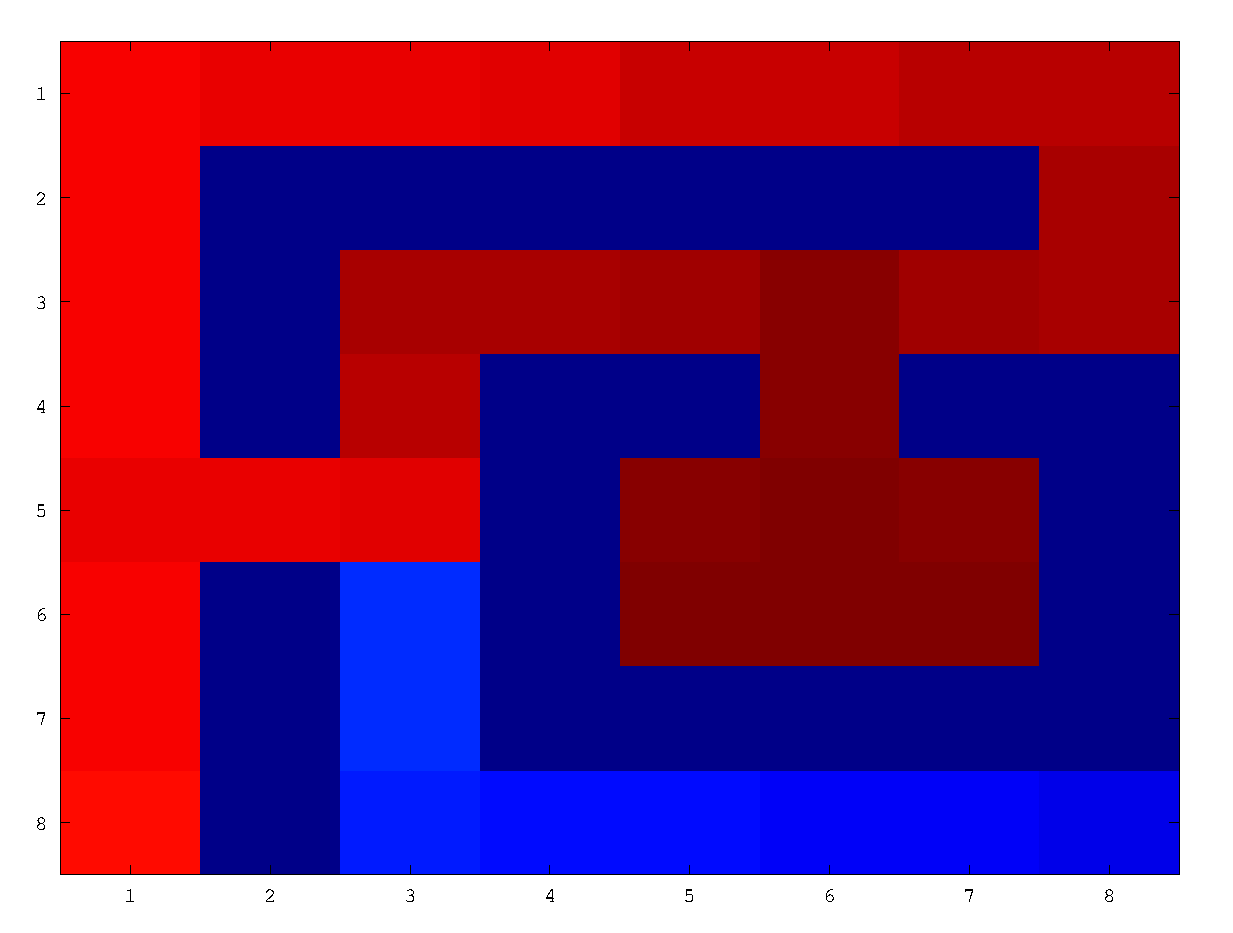
\includegraphics[width=0.45\textwidth]{pit_random_0_1}}
    \subfigure[$\omega = 0.5$]{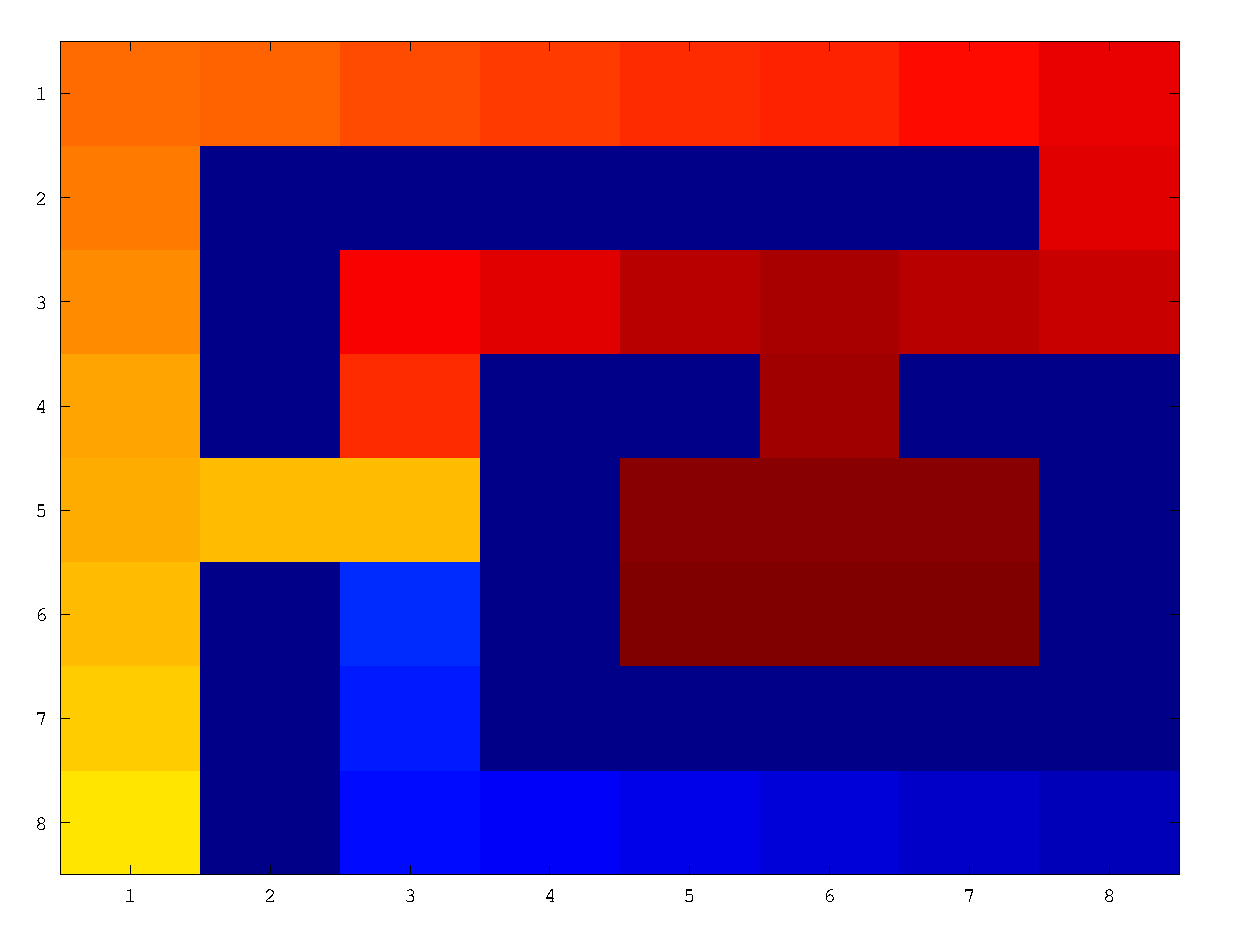
\includegraphics[width=0.45\textwidth]{pit_random_0_5}}
    \subfigure[value]{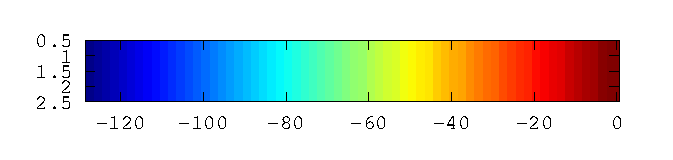
\includegraphics[width=0.45\textwidth]{color-axis}}
    \caption{Pit maze solutions for two values of $\omega$.}
    \label{fig:pit-solution}
  \end{figure}
Randomness changes the solution significantly in this environment. When $\omega$ is relatively small, it is worthwhile (in expectation) for the agent to pass past the pit, even though there is a risk of falling in and getting a reward of $-100$. In the example given, even starting from the third row, the agent prefers taking the short-cut. For high enough $\omega$, the optimal policy avoids approaching the pit. Still, the agent prefers jumping in the pit, than being trapped at the bottom of the maze forever.


\subsubsection{Continuing problems}
Finally, many problems have no natural terminating state, but are continuing \emph{ad infinitum}. Frequently, we model those problems using a utility that discounts future rewards exponentially. This way, we can guarantee that the utility is bounded. In addition, exponential discounting also has some economical sense. This is partially because of the effects of inflation, and partially because money now may be more useful than money in the future. Both these effects diminish the value of money over time.  As an example, consider the following inventory management problem. 

\begin{example}[Inventory management]
  There are $K$ storage locations, and each location $i$ can store
  $n_i$ items.  At each time-step there is a probability $\phi_i$ that
  a client tries to buy an item from location $i$, where $\sum_i
  \phi_i \leq 1$.  If there is an item available, when this happens,
  you gain reward $1$.  There are two types of actions, one for
  ordering a certain number $u$ units of stock, paying $c(u)$.
  Further one may move $u$ units of stock from one location $i$ to
  another location $j$, paying $\psi_{ij}(u)$.
\end{example}

An easy special case is when $K=1$, and we assume that deliveries
happen once every $m$ timesteps, and each time-step a client arrives
with probability $\phi$.  Then the state set $\CS=\{0, 1, \ldots, n
\}$ corresponds to the number of items we have, the action set
$\CA=\{0, 1, \ldots, n\}$ to the number of items we may order.  The
transition probabilities are given by $P(s'|s,a) =
\binom{m}{d}\phi^d(1-\phi)^{m-d}$, where $d=s+a-s'$, for $s+a \leq n$.
  % ro: What's the solution?
  % cd: I guess I should try and give the solution to this problem for these special cases.


\newcommand{\Node}[3]{%
  \pgfnodecircle{#1}[stroke]{#2}{0.3cm}%
  \pgfputat{\pgfrelative{#2}{\pgfxy(0,-.075)}}{\pgfbox[center,base]{#3}}}

\newcommand{\SNode}[3]{%
  \pgfnodebox{#1}[stroke]{#2}{0.3cm}%
  \pgfputat{\pgfrelative{#2}{\pgfxy(0,-.075)}}{\pgfbox[center,base]{#3}}}

\newcommand{\BNode}[3]{%
  \pgfnodecircle{#1}[stroke]{#2}{0.4cm}%
  \pgfputat{\pgfrelative{#2}{\pgfxy(0,-.075)}}{\pgfbox[center,base]{#3}}}

\newcommand{\Claim}[2]{%
  \pgfputat{\pgfrelative{\pgfxy(0.4,-0.075)}{\pgfnodecenter{#1}}}%
  {\pgfbox[left,base]{#2}}}

\newcommand{\LClaim}[2]{%
  \pgfputat{\pgfrelative{\pgfxy(-0.4,-0.075)}{\pgfnodecenter{#1}}}%
  {\pgfbox[right,base]{#2}}}

\newcommand{\Bush}[3]{%
  \pgfnodecircle{#1}[virtual]{\pgfrelative{\pgfnodecenter{#2}}{#3}}{1pt}%
  \pgfnodeconnline{#2}{#1}}


\subsection{Markov chain theory for discounted problems}
\label{sec:markov-chain-theory}
  Here we consider MDPs with infinite horizon and discounted rewards. We shall consider undiscounted rewards only in Chapter~\ref{cha:distr-free-reinf}.
  Our utility in this case is the discounted total reward:
  \[
  U_t = \lim_{T\to \infty} \sum_{k=t}^T \disc^k r_k, \qquad \disc \in (0,1)
  \]
For simplicity, in the following we assume that rewards only depend on the current state instead of both state and action. It can easily be verified that results still hold in the latter case. More importantly, we also assume that the state and action spaces $\CS, \CA$ are finite, and that the transition kernel of the MDP is time-invariant. This allows us to use the following simplified vector notation:
\begin{itemize}
\item $\val^\pol = \left(\E^\pol(U_t \mid s_t = s)\right)_{s \in \CS}$ is a vector in $\Reals^{|\CS|}$ representing the value of policy $\pol$.
\item Sometimes we will use $p(j|s,a)$ as a shorthand for $\Pr_{\mdp}(s_{t+1} = j \mid s_t = s, a_t = a)$.
\item $\trans_{\mdp,\pol}$ is a transition matrix in $\Reals^{|\CS|\times|\CS|}$ for policy $\pol$, such that
  \[
  \trans_{\mdp,\pol}(i,j) = \sum_a p(j \mid i, a) \Pr^\pol(a \mid i).
  \]
\item $\rew$ is a reward vector in $\Reals^{|\CS|}$.
\item The space of value functions $\Vals$ is a Banach space \only<article>{(i.e., a complete, normed vector space)} equipped with the norm
  \[
  \|\val\| = \sup\cset{|\val(s)|}{s \in \CS}
  \]
  
\end{itemize}
  \only<article>{For infinite-horizon discounted MDPs, stationary policies are sufficient. This can be proven by induction, using arguments similar to other proofs given here. For a detailed set of proofs, see~\cite{Puterman:MDP:1994}.}
  \begin{definition}
    A policy $\pol$ is stationary if $\pol(a_t \mid s_t) = \pol(a_n \mid s_n)$ for all $n, t$. %ro: can't understand notation nor definition
    \label{def:stationary-policy}
  \end{definition}
  \only<article>{We now present a set of important results that link Markov decision processes to linear algebra.}
  \begin{remark}
    We can use the Markov chain kernel $\trans$ to write the expected reward vector as
    \begin{align}
      \val^\pol
      &=
      \sum_{t=0}^\infty \disc^{t} \trans_{\mdp,\pol}^{t} \rew
      \label{eq:kernel-value}
    \end{align}
    \label{rem:kernel-value}
  \end{remark}
  \only<article>{
    \begin{proof}
      \begin{align*}
        V^\pol(s)
        &= \E \left(\sum_{t=0}^\infty \disc^t r_t ~\middle|~ s_0 = s\right)
        \\
        &= \sum_{t=0}^\infty \disc^t \E(r_t | s_0 = s)
        \\
        &= \sum_{t=0}^\infty \disc^t \sum_{i \in \CS} \Pr(s_t = i \mid s_0 = s) \E(r_t \mid s_t = i).
      \end{align*}
      Since for any distribution vector $\vectorsym{p}$ over $\CS$, we have $\E_\vectorsym{p} r_t = \transpose{\vectorsym{p}} \rew$, the result follows.%ro: Actually, you need some knowledge about the power of the transition matrix, right?
    \end{proof}
  }

  It is possible to show that the expected discounted total reward of a policy is equal to the expected undiscounted total reward with a geometrically distributed horizon (see exercise~\ref{exercise:geometric-discounting}. As a corollary, it follows a Markov decision process with discounting is equivalent with one where there is no discounting, but a stopping probability $(1 - \disc)$ at every step.

The value of a particular policy can be expressed as a linear equation. This is an important result, as it has led to a number of successful algorithms that employ linear theory.
  \begin{theorem}
    For any stationary policy $\pol$, $\val^\pol$ is the unique solution of
    \begin{equation}
      \label{eq:bellman-equation}
      \val = \rew + \disc \trans_{\mdp,\pol} \val. \only<presentation>{\quad \leftarrow \textrm{fixed point}}
    \end{equation}
    In addition, the solution is:
    \begin{equation}
      \label{eq:bellman-solution}
      \val^\pol = (\ident - \disc \trans_{\mdp,\pol})^{-1} \rew,
    \end{equation}
    \label{the:inverse-value}
    where $\ident$ is the identity matrix.
  \end{theorem}

    To prove this we will need the following important theorem. 
    \begin{theorem}\label{thm:wert}
      For any bounded linear transformation $\matrixsym{A} : S \to S$ on a normed
      linear space $S$ (i.e., there is $c < \infty$ s.t. $\|\matrixsym{A}x\|:=\sup_i \sum_j a_{i,j} \leq c\|x\|$ for all $x \in S$ with \emindex{spectral radius}
      $\sigma(\matrixsym{A}) \defn \lim_{n\to \infty} \|\matrixsym{A}^n\|^{1/n} < 1$), $\matrixsym{A}^{-1}$ exists and is given by
      \begin{equation}
        \matrixsym{A}^{-1} = \lim_{T \to \infty} \sum_{n=0}^T (\ident - \matrixsym{A})^n.
      \end{equation}
    \end{theorem}

  \begin{proof}[Proof of Theorem~\ref{the:inverse-value}]
    First note that by manipulating the infinite sum in Remark~\ref{rem:kernel-value}, one obtains $\rew = (\ident - \disc \trans_{\mdp,\pol}) \val^\pol$.
    Since $\|\disc \trans_{\mdp,\pol}\| < 1 \cdot \|\trans_{\mdp_\pol}\| = 1$, the inverse 
    \[
    (\ident - \disc \trans_{\mdp,\pol})^{-1} = \lim_{n \to \infty} \sum_{t=0}^n (\disc \trans_{\mdp,\pol})^t
    \]
    exists by Theorem \ref{thm:wert}.
    It follows that
    \[
    \val = (\ident - \disc \trans_{\mdp,\pol})^{-1} \rew
    = \sum_{t=0}^\infty \disc^t \trans_{\mdp,\pol}^t \rew = \val^\pol,
    \]
    where the last step is by Remark~\ref{rem:kernel-value} again.%ro: do we need to argue for uniqueness of the solution?
  \end{proof}
It is important to note that the matrix $\matrixsym{X} = (\ident - \disc \trans_{\mdp,\pol})^{-1}$ can be seen as the expected number of discounted cumulative visits to each state $s$, starting from state $s'$ and following policy $\pol$. More specifically, the entries of the matrix are:
\begin{equation}
x(s,s') = \E^\pol_\mdp
\left\{
  \sum_{t=0}^\infty \gamma^t \Pr_\mdp^\pol(s_t = s' \mid s_t = s)
\right\}.
\label{eq:cumulative-visits}
\end{equation}
This interpretation is quite useful, as many algorithms rely on an estimation of $\matrixsym{X}$ for approximating value functions.

\subsection{Optimality equations}
\label{sec:optimality-equations}
\only<article>{Let us now look at the backwards induction algorithms in terms of operators. We introduce the operator of a policy, which is the one-step backwards induction operation for a fixed policy, and the Bellman operator, which is the equivalent operator for the optimal policy. If a value function is optimal, then it satisfies the Bellman optimality equation.}
\begin{frame}
  \begin{definition}[Policy and Bellman operator]
    \only<article>{The linear operator of a policy $\pol$ is:}
    \begin{equation}
      \blm_\pol \val \defn\rew + \disc \trans_\pol \val %ro: Here, the mu is dropped. Maybe we should drop it already earlier. % cd: hm, ok, maybe that makes sense
      \label{eq:policy-operator}
    \end{equation}
    Sby contract    \only<article>{The (non-linear) Bellman operator in the space of value functions $\Vals$ is defined as:}
    \begin{equation}
      \blm \val \defn \sup_\pol \set{\rew + \disc \trans_\pol \val}, \qquad \val \in \Vals
      \label{eq:bellman-operator}
    \end{equation}    
    \label{def:bellman-operator}
  \end{definition}
  \only<article>{
    We now show that the Bellman operator satisfies the following monotonicity properties with respect to an arbitrary value vector $\val$.
  }
  \begin{theorem}
    Let $\val^* \defn \sup_\pol \val^\pol$. Then for any bounded $\rew$, it holds that for $\val \in \Vals$:
    \begin{itemize}
    \item[(1)] If $\val \geq \blm \val$, then $\val \geq \val^*$.
    \item[(2)] If $\val \leq \blm \val$, then $\val \leq \val^*$.
    \item[(3)] If $\val = \blm \val$, then $\val$ is unique and $\val = \sup_\pol \val^\pol$.
      Therefore, $\val = \blm \val$ is called the Bellman optimality equation.
    \end{itemize}
  \end{theorem}
  \only<article>{
    \begin{proof}
      We first prove (1). A simple proof by induction over $n$ %ro: Is there an easier way to see this?
      shows that for any $\pol$
      \begin{align*}
        \val
        &\geq
        \rew + \disc \trans_\pol \val
        \geq
        \sum_{k=0}^{n-1}\disc^k\trans_\pol^k\rew
        + \disc^n \trans_\pol^n \val.
      \end{align*}
      Since $\val^\pol = \sum_{t=0}^\infty \disc^t \trans^t_\pol \rew$ it follows that
      \[
      \val - \val^\pol 
      \geq
      \disc^n \trans_\pol^n \val
      -\sum_{k=n}^{\infty}\disc^k\trans_\pol^k\rew.
      \]
      The first-term on the right-hand side can be bounded by arbitrary $\epsilon/2$ for large enough $n$. Also note that %ro: I'm confused by the second part of the proof. Shouldn't we have lower bounds for the terms here to get what we want?
      \[
      \sum_{k=n}^{\infty}\disc^k\trans_\pol^k\rew \geq -\frac{\disc^n \vectorsym{e}}{1 - \disc},
      \]
      with $\vectorsym{e}$ being a unit vector, so this can be bounded by $\epsilon/2$ as well. So for any $\pol, \epsilon > 0$:
      \[
      \val \geq \val^\pol - \epsilon,
      \]
      so
      \[
      \val \geq \sup_\pol \val^\pol.
      \]
      An equivalent argument shows that
      \[
      \val \leq \val^\pol + \epsilon,
      \]
      proving (2).
      Putting together (1) and (2) gives (3).
    \end{proof}
  }
\end{frame}


\begin{frame}
  \only<article>{
    We eventually want show that repeated application of the Bellman operator converges to the optimal value.
    As a preparation, we need the following theorem. 
  }
  \begin{theorem}[Banach Fixed-Point theorem]
    Suppose $\CS$ is a Banach space (i.e. a complete normed linear space) and $T : \CS \to \CS$ %ro: Using \CS here is quite unfortunate, as this usually denotes the state space, which is a bit confusing at the beginning of the next proof.
    is a contraction mapping (i.e. $\exists \disc \in [0,1)$ s.t. $\|Tu-Tv\| \leq \disc \|u-v\|$ for all $u,v \in \CS$). Then
    \begin{itemize}
    \item there is a unique $u^* \in U$ s.t. $Tu^* = u^*$, and
    \item for any $u^0 \in \CS$ the sequence $\{u^n\}$:
      \[
      u^{n+1}  = Tu^{n} = T^{n+1} u^0
      \]
      converges to $u^*$.
    \end{itemize}
    \label{the:fixed-point}
  \end{theorem}
  \begin{proof}
    For any $m \geq 1$
    \begin{align*}
      \|u^{n+m} - u^{n}\|
      &\leq
      \only<1->{
        \sum_{k=0}^{m-1} \|u^{n+k+1} - u^{n + k}\|
        =
        \sum_{k=0}^{m-1} \|T^{n+k}u^{1} - T^{n+k}u^{0}\|
      }
      \only<2->{
        \\
        &\leq
        \sum_{k=0}^{m-1} \disc^{n+k} \|u^{1} - u^{0}\|
        = 
        \frac{\disc^n(1 - \disc^m)}{1 - \disc}\|u^1 - u^0\|.  %ro: A few words why this is sufficient would be in order.
      }
    \end{align*}
  \end{proof}
\end{frame}

\begin{frame}
  \begin{theorem}
    For $\disc \in [0,1)$ the Bellman operator $\blm$ is a contraction mapping in $\Vals$.
    \label{the:bellman-contraction}
  \end{theorem}
  \begin{proof}
    Let $\val, \val' \in \Vals$. Consider $s \in \CS$ such that $\blm \val(s) \geq \blm \val'(s)$, and let
    \[
    a^*_s \in \argmax_{a \in \CA} \set{r(s) + \sum_{j \in \CS} \disc p_\mdp(j\mid s, a) \val(j)}.
    \]
    Using the fact that $a^*_s$ is optimal for $\val$, but not necessarily for $\val'$, we have:
    \begin{align*}
      0
      &\leq
      \blm \val(s) - \blm \val'(s)
      \leq  
      \only<article>{
        \sum_{j \in S} \disc p(j \mid s, a^*_s) \val(j)
        -
        \sum_{j \in S} \disc p(j \mid s, a^*_s) \val'(j)
        \\
        &=
        \disc \sum_{j \in S}  p(j \mid s, a^*_s) [\val(j) - \val'(j)]
        \\
        &\leq 
        \disc \sum_{j \in S}  p(j \mid s, a^*_s) \|\val - \val'\|
        =
      }
      \disc \|\val - \val'\|.
    \end{align*}
    Repeating the argument for $s$ such that $\blm \val(s) \leq \blm \val'(s)$, we obtain
    \[
    |\blm \val (s) - \blm \val'(s)| \leq \disc\|\val - \val'\|.
    \]
    Taking the supremum over all possible $s$, the required result follows.
  \end{proof}
  It is easy to show the same result for the $\blm_\pol$ operator, as a corollary to this theorem.
\end{frame}

\begin{frame}
  \begin{theorem}
    For discrete $\CS$, bounded $\rew$, and $\disc \in [0,1)$
    \begin{enumerate}[(i)]
    \item there is a unique $\val^* \in \Vals$ such that $\blm \val^* = \val^*$ and such that $\val^* = V^*_\mdp$,
    \item for any stationary policy $\pol$, there is a unique $\val \in \Vals$ such that $\blm_\pol \val = \val$ and $\val = V^\pol_\mdp$.
    \end{enumerate}
    \label{the:bellman-convergence}
  \end{theorem}
  \only<article>{
    \begin{proof}
      As the Bellman operator $\blm$ is a contraction by Theorem~\ref{the:bellman-contraction}, application of the fixed-point Theorem \ref{the:fixed-point}
      shows that there is a unique $\val^* \in \Vals$ such that $\blm \val^* = \val^*$. This is also the optimal value function due to Theorem~\ref{the:bellman-contraction}.%ro: The latter reference seems to be wrong, but I'm not sure what's the correct reference.
      The second part of the theorem follows from the first part when considering only a single policy $\pi$ (which then is optimal).
      % Use part 1 with $\Pols = \{\pol\}$.  %ro: \Pol hasn't been used in this section so far.
    \end{proof}
  }
\end{frame}

\subsection{MDP Algorithms}
\label{sec:mdp-algorithms}
\only<article>{Let us now look at three basic algorithms for solving a known Markov decision process. The first, \textit{value iteration}\index{value iteration}, is a simple extension of the backwards induction algorithm to the infinite horizon case. %This is possible to do, since the value converges and consequently we do not need to store all value vectors. %ro: outcommented this: also for backwards induction you need not store all the values, so didn't understand this
}
\subsubsection{Value iteration}
In this version of the algorithm, we assume that rewards are dependent only on the state. An algorithm for the case where reward only depends on the state can be obtained by replacing $r(s,a)$ with $r(s)$.
\label{sec:value-iteration}
\begin{frame}
  \begin{algorithm}[H]
    \begin{algorithmic}
      \STATE Input $\mdp$, $\CS$.
      \STATE Initialise $\val_0 \in \Vals$. %ro: What is \Vals here?
      \FOR{$n=1, 2, \ldots$}
      \FOR{$s \in \CS_n$}
      \STATE $\pol_n(s) = \argmax_{a \in \CA} \set{r(s, a) + \disc \sum_{s' \in \CS} P_\mdp(s' \mid s, a) \val_{n-1} (s')}$
      \STATE $\val_n(s) = r(s, \pol_n(s)) + \disc \sum_{s' \in \CS} P_\mdp(s' \mid s, \pol_n(s)) \val_{n-1} (s')$
      \ENDFOR
      \STATE \textbf{break} if \texttt{termination-condition} is met %ro: what is this condition?
      \ENDFOR
      \STATE Return $\pol_n, V_n$.
    \end{algorithmic}
    \caption{Value iteration}
  \end{algorithm}
\end{frame}

  The value iteration algortihm is a direct extension of the backwards induction algorithm for an infinite horizon. However, since we know that stationary policies are optimal, we do not need to maintain the values and actions for all time steps. At each step, we can merely keep the previous value $\val_{n-1}$. However, since there is an infinite number of steps, we need to know whether the algorithm converges to the optimal value, and what is the error we make at a particular iteration.
  \begin{theorem}
    The value iteration algorithm satisfies
    \begin{itemize}
    \item $\lim_{n \to \infty} \|\val_n - \val^*\| = 0$. 
    \item For each $\epsilon>0$ there exists $N_\epsilon <\infty$ such that for all $n\geq N_\epsilon$
      \begin{equation}
        \|\val_{n+1} - \val_n\| \leq \epsilon(1 - \disc)/2\disc.
        \label{eq:value-iteration-stopping}
      \end{equation}
    \item For $n\geq N_\epsilon$ the policy $\pol_\epsilon$ that takes action
      \[
      \argmax_a r(s,a) + \disc \sum_j p(j|s,a)\val_n(s')
      \]
      is
      $\epsilon$-optimal, i.e. $V^{\pol_\epsilon}_\mdp(s) \geq V^*_\mdp(s) - \epsilon$ for all states $s$.
    \item $\|\val_{n+1} - \val^*\| < \epsilon/2$ for $n \geq N_\epsilon$.
    \end{itemize}
  \end{theorem}
  \begin{proof}
    The first two statements follow from the fixed-point Theorem \ref{the:fixed-point}.
    Now note that
    \[
    \|V^{\pol_\epsilon}_\mdp - \val^*\|
    \leq
    \|V^{\pol_\epsilon}_\mdp - \val_n\|
    +
    \|\val_n - \val^*\|
    \]
    We can bound these two terms easily:  %ro: Some explanations would be helpful. Actually, I only understand the first equality. % cd: I had typos!
    \only<article>{
      \begin{align*}
        \norm{V^{\pol_\epsilon}_\mdp - \val_{n+1}}
        &= 
        \norm{\blm_{\pol_\epsilon} V^{\pol_\epsilon}_\mdp - \val_{n+1}}
        \tag{by definition of $\blm_{\pol_\epsilon}$}
        \\
        &\leq 
        \norm{\blm_{\pol_\epsilon} V^{\pol_\epsilon}_\mdp - \blm \val_{n+1}}
        +
        \norm{\blm \val_{n+1} - \val_{n+1}}
        \tag{triangle}
        \\
        &=
        \norm{\blm_{\pol_\epsilon} V^{\pol_\epsilon}_\mdp - \blm_{\pol_\epsilon} \val_{n+1}}
        +
        \norm{\blm \val_{n+1} - \blm \val_{n}}
        \tag{by definition}
        \\
        &\leq
        \disc \norm{V^{\pol_\epsilon}_\mdp - \val_{n+1}}
        +
        \disc \norm{\val_{n+1} -\val_{n}}.
        \tag{by contraction}
      \end{align*}
      An analogous argument gives the same bound for the second term  $\|\val_n - \val^*\|$. Then, rearranging we obtain
    }
    \[
    \norm{V^{\pol_\epsilon} - \val_{n+1}} 
    \leq
    \frac{\disc}{1 - \disc}\|\val_{n+1} - \val_{n}\|,
    \qquad
    \|\val_{n+1} - \val^*\|
    \leq
    \frac{\disc}{1 - \disc}\|\val_{n+1} - \val_{n}\|,
    \]
    and the third and fourth statements follow from the second statement.
  \end{proof}

  The \emindex{termination condition} of value iteration has been left unspecified. However, the theorem above shows that if we terminate when \eqref{eq:value-iteration-stopping} is true, then our error will be bounded by $\epsilon$. However, better termination conditions can be obtained.

Now let us prove how fast value iteration converges.
  \begin{theorem}[Value iteration monotonicity]
    Let $\Vals$ be the set of value vectors with Bellman operator $\blm$. Then:
    \begin{enumerate}
    \item Let $\val, \val' \in \Vals$ with $\val' \geq \val$. Then $\blm
      \val' \geq \blm \val$.
    \item Let $\val_{n+1} = \blm \val_n$. If there is an $N$ s.t.\ $\blm
      \val_N \leq \val_N$, then $\blm \val_{N+k} \leq \val_{N+k}$ for
      all $k \geq 0$ and similarly for $\geq$.
    \end{enumerate}
    \label{the:value-iteration-monotonicity}
  \end{theorem}
  \begin{proof}
    Let $\pol \in \argmax_\pol \rew + \disc \trans_{\mdp,\pol} \val$. Then
    \[
    \blm \val
    = \rew + \disc \trans_{\mdp,\pol} \val
    \leq \rew + \disc \trans_{\mdp,\pol} \val'
    \leq \max_{\pol'}\rew + \disc \trans_{\mdp,\pol'} \val',
    \]
    where the first inequality is due to the fact that $\trans \val \geq \trans \val'$ for any $\trans$.
    For the second part, 
    \[
    \blm \val_{N+k} = \val_{N+k+1} = \blm^k \blm \val_N \leq \blm^k \val_N = \val_{N+k}.
    \]
    since $\blm \val_N \leq \val_N$ by assumption and consequently $\blm^k \blm \val_N \leq \blm^k \val_N$ by part one of the theorem.
  \end{proof}

  Thus, value iteration converges monotonically to $V^*_{\mdp}$ if the
  initial value $\val_0 \leq \val'$ for all $\val'$.  If $r \geq 0$,
  it is sufficient to set $\val_0 = \mathbf{0}$. Then $\val_n$ is always
  a lower bound on the optimal value function.
\begin{theorem}
  Value iteration converges with error in $O(\disc^n)$
  More specifically, for $r \in [0,1]$ and $\val_0 = \mathbf{0}$, 
  \begin{align*}
    \|\val_n - V_\mdp^*\| &\leq \frac{\disc^n}{1 - \disc},
    &
    \|V^{\pol_n}_\mdp - V_\mdp^*\| &\leq \frac{2\disc^n}{1 - \disc}.
  \end{align*}
\end{theorem}
\begin{proof}
  The first part follows from the contraction property (Theorem~\ref{the:bellman-contraction}):
  \begin{equation}
    \|\val_{n+1} - \val^*\|
    =
    \|\blm \val_{n} - \blm \val^*\|
    \leq 
    \disc \|\val_{n} - \val^*\|.  %ro: This proves the convergence rate, what about the inequalities? 
  \end{equation}
  Now divide by $\disc^n$ to obtain the final result.
  
\end{proof}

Although value iteration converges exponentially fast, the convergence
is dominated by the discount factor $\disc$. When $\disc$ is very
close to one, convergence can be extremely slow.  In fact,
\citet{tseng1990solving} showed that the number of iterations are on
the order of $1 / (1 - \disc)$, for bounded accuracy of the input
data. The overall complexity is
$\tilde{O}(|\CS|^2 |\CA| L (1 - \disc)^{-1}$, omitting logarithmic
factors, where $L$ is the total number of bits used to represent the
input.\footnote{Thus the result is \emph{weakly} polynomial complexity, due to the dependence on the input size description.}

\subsubsection{Policy iteration}
\label{sec:policy-iteration}
\index{policy iteration}
Unlike value iteration, \textit{policy iteration} attempts to iteratively improve a given policy, rather than a value function. At each iteration, it calculates the value of the current policy and then  calculates the policy that is greedy with respect to this value function. For finite MDPs, the policy evaluation step can be performed with either linear algebra or backwards induction, while the policy improvement step is trivial. The algorithm described below can be extended to the case when the reward also depends on the action, by replacing $\rew$ with the policy-dependent reward vector $\rew_\pol$. 

\begin{algorithm}[H]
  \begin{algorithmic}
    \STATE Input $\mdp$, $\CS$.
    \STATE Initialise $\val_0$.
    \FOR{$n=1, 2, \ldots$}
    \STATE $\pol_{n+1} = \argmax_\pol \set{\rew + \disc \trans_\pol \val_n}$ \qquad \texttt{ // policy improvement}  
    \STATE $\val_{n+1} = V^{\pol_{n+1}}_\mdp$ \qquad \texttt{ // policy evaluation}  
    \STATE \textbf{break} if $\pol_{n+1} = \pol_n$.
    \ENDFOR
    \STATE Return $\pol_n, \val_n$.
  \end{algorithmic}
  \caption{Policy iteration}
  \label{alg:policy-iteration}
\end{algorithm}


The following theorem describes an important property of policy iteration, namely that the policies generated are monotonically improving.

\begin{theorem}
  Let $\val_n, \val_{n+1}$ be the value vectors generated by policy iteration.
  Then $\val_n \leq \val_{n+1}$.
\end{theorem}
\begin{proof}
  From the policy improvement step
  \[
  \rew + \disc \trans_{\pol_{n+1}} \val_n
  \geq
  \rew + \disc \trans_{\pol_{n}} \val_n,
  = \val_n
  \]
  where the equality is due to the policy evaluation step for $\pol_{n}$. Rearranging, we get $ \rew \geq (\ident - \disc \trans_{\pol_{n+1}}) \val_n$
  and hence
  \begin{align*}
    (\ident - \disc \trans_{\pol_{n+1}})^{-1} \rew &\geq \val_n,
  \end{align*}
  noting that the inverse is positive. 
  Since the left side equals $\val_{n+1}$ by the policy evaluation step for $\pol_{n+1}$, the theorem follows.
\end{proof}
We can use the fact that the policies are monotonically improving to show that policy iteration will terminate after a finite number of steps.
\begin{corollary}
  If $\CS, \CA$ are finite, then policy iteration terminates after a finite number of iterations and returns an optimal policy.
\end{corollary}

\begin{proof}
  There is only a finite number of policies, and since policies in policy iteration are monotonically improving, the algorithm must stop after finitely many iterations.
  Finally, the last iteration satisfies
  \begin{equation}
    \val_n = \max_\pol \rew + \disc \trans_\pol \val_n.
  \end{equation}
  Thus $\val_n$ solves the optimality equation.
\end{proof}

However, it is easy to see that the number of policies is $|\CA|^{|\CS|}$, thus the above corollary only guarantees exponential-time convergence in the number of states. However, it is also known that the complexity of policy iteration is strongly polynomial~\cite{ye2011simplex}, for any fixed $\disc$, with the number of iterations required being $\frac{|\CS|^2 (|\CA| - 1)}{1 - \disc} \cdot \ln \left( \frac{|\CS|^2}{1 - \disc} \right)$.

Policy iteration seems to have very different behaviour from value iteration. In fact, one can obtain families of algorithms that lie at the extreme ends of the spectrum between policy iteration and value iteration. The first member of this family is modified policy iteration, and the second member is temporal difference policy iteration.


\subsubsection{Modified policy iteration}
\index{policy iteration!modified}
The astute reader will have noticed that it may be
not necessary to fully evaluate the improved
policy. In fact, we can take advantage of that to speed up policy iteration. Thus, a simple variant of policy iteration involves doing only a $k$-step update for the policy evaluation step. For $k=1$, the algorithm becomes identical to value iteration, while for $k \to \infty$ the algorithm is equivalent to policy iteration, as $\val_n = V^{\pol_n}$.
\begin{algorithm}[H]
  \begin{algorithmic}
    \STATE Input $\mdp$, $\CS$.
    \STATE Initialise $\val_0$.
    \FOR{$n=1, 2, \ldots$}
    \STATE $\pol_{n} = \argmax_\pol \rew + \disc \trans_\pol \val_{n-1}$ \qquad \texttt{ // policy improvement}  
    \STATE $\val_{n} = \blm_{\pol_{n}}^k \val_{n-1}$ \qquad \texttt{// partial policy evaluation}
    \STATE \textbf{break} if $\pol_{n} = \pol_{n+1}$.
    \ENDFOR
    \STATE Return $\pol_n, \val_n$.
  \end{algorithmic}
  \caption{Modified policy iteration}
\end{algorithm}
Modified policy iteration can perform much better than either pure value iteration or pure policy iteration.
\subsubsection{A geometric view}
\index{temporal differences}
It is perhaps interesting to see the problem from a geometric perspective. This also gives rise to the so-called ``temporal-difference'' set of algorithms.
First, we define the difference operator, which is the difference between a value function vector $\val$ and its transformation via the Bellman operator.
\begin{definition}
  The \emindex{difference operator} is defined as 
  \begin{equation}
    \label{eq:td-operator}
    \pim \val \defn \max_\pol \set{\rew + (\disc \trans_\pol - \ident) \val} = \blm \val - \val.
  \end{equation}
  \label{def:td-operator}
\end{definition}
Essentially, it is the change in the value function vector when we apply the Bellman operator. 
Thus the Bellman optimality equation can be rewritten as
\begin{equation}
  \label{eq:td-equation}
  \pim \val = \textbf{0}.
\end{equation}
Now let us define the set of greedy policies with respect to a value vector  $\val \in \Vals$ to be:
\[
\Pols_\val \defn \argmax_{\pol \in \Pols} \set{\rew + (\disc \trans_\pol - \ident)\val}.
\]
We can now show the following inequality between the two different value function vectors.
\begin{theorem}
  For any $\val, \val' \in \Vals$ and $\pol \in \Pols_\val$
  \begin{equation}
    \label{eq:td-support}
    \pim \val' \geq \pim \val + (\disc \trans_\pol - \ident)(\val' - \val).
  \end{equation}
\end{theorem}
\begin{proof}
  By definition, $\pim \val' \geq \rew + (\disc \trans_\pol - \ident)\val'$,
  while $\pim \val = \rew + (\disc \trans_\pol - \ident)\val$. Subtracting the latter from the former gives the result.
\end{proof}
Equation \eqref{eq:td-support} is similar to the convexity of the Bayes-optimal utility \eqref{eq:convex-bayes-util}. 
Geometrically, we can see from a look at Figure~\ref{fig:difference-operator}, that applying the Bellman operator on value function always improves it, yet may have a negative effect on the other value function. If the number of policies is finite, then the figure is also a good illustration of the policy iteration algorithm, where each value function improvement results in a new point on the horizontal axis, and the choice of the best improvement (highest line) for that point. In fact, we can write the policy iteration algorithm in terms of the difference operator.

\begin{figure}[ht]
  \centering
  \if 0
  \begin{tikzpicture}[
      pnt/.style={
        circle,
        fill=black,
        thick,
        inner sep=2pt,
        minimum size=0.1cm
      }
    ] 
    \node at (0,0) (start) {};
    \node at (2,0) (vs) [pnt,label=below:$\val^*$] {};
    \node at (5,0) (v1) [pnt,label=below:$\val$] {};
    \node at (8,0) (v2) [pnt,label=below:$\val'$] {};
    \node at (10,0) (end)  {};
    \draw (start) -- (end);
    \node at (8,1) (Bs2) {};
    \node at (8,2) (B2) {};
    \node at (2,-1) (B2s) {};
    \draw (Bs2) -- (vs);
    \draw (B2) -- (B2s);
  \end{tikzpicture}
  \fi
  \input{figures/difference-operator.tikz}
  \caption{The difference operator. The graph shows the effect of the operator for the optimal value function $\val^*$, and two arbitrary value functions, $\val_1, \val_2$. Each line is the improvement effected by the greedy policy $\pol^*, \pol_1, \pol_2$ with respect to each value function $\val^*, \val_1, \val_2$. }
  \label{fig:difference-operator}
\end{figure}
\begin{theorem}
  Let $\{\val_n\}$ be the sequence of value vectors obtained from policy iteration. Then for any $\pol \in \Pols_{\val_n}$,
  \begin{equation}
    \val_{n+1} = \val_n - (\disc \trans_{\pol} - \ident)^{-1} \pim \val_n.
  \end{equation}
\end{theorem}
\begin{proof}
  By definition, we have for  $\pol \in \Pols_{\val_n}$
  \begin{align*}
    \val_{n+1} 
    &=
    (\ident - \disc \trans_\pol)^{-1} \rew - \val_n + \val_n
    \\
    &=
    (\ident - \disc \trans_\pol)^{-1} [
    \rew - (\ident - \disc \trans_\pol)\val_n] + \val_n.
  \end{align*}
  Since $\rew - (\ident - \disc \trans_\pol)\val_n = \pim \val_n$ the claim follows.
\end{proof}


\subsubsection{Temporal-Difference Policy Iteration}
\index{policy iteration!temporal-difference} \index{temporal
  difference} 

 In \emph{temporal-difference policy iteration},
similarly to the modified policy iteration algorithm, we replace the
next-step value with an approximation $\val_n$ of the $n$-th policy's
value. Informally, this approximation is chosen so as to reduce the
discrepancy of our value function over time.

At the $n$-th iteration of the algorithm, we use a policy improvement step to obtain the next policy $\pol_{n+1}$ given our current approximation $\val_n$:
\begin{equation}
  \blm_{\pol_{n+1}} \val_n = \blm \val_n.
\end{equation}
To update the value from $\val_n$ to $\val_{n+1}$ we rely on the \emindex{temporal difference error}, defined as:
\begin{equation}
  d_n(i,j) = [\rew(i) + \disc \val_n(j)] - \val_n(i).
\end{equation}
This can be seen as the difference in the estimate
when we move from state $i$ to state $j$. In fact, it is easy to see that, if our value function estimate satisfies $\val = V^{\pol_n}$, then the expected error should be zero, as:
\[
\sum_{j \in \CS} d_n(i,j) p(j \mid i, \pol_n (i)) = 
\sum_{j \in \CS} [\rew(i) + \disc \val_n(j)] p(j \mid i, \pol_n(i))
-\val_{n}(i).
\]
Note the similarity to the difference operator in modified policy iteration.  The idea of the temporal-difference policy iteration is to use adjust the current value $\val_n$, using the temporal differences mixed over an infinite number of steps:
\begin{align}
  \vectorsym{\tau}_n(i) &= \sum_{t=0}^\infty \E_{\pol_n} \left[(\disc \lambda)^t d_n(s_t,s_{t+1}) \mid s_0 = i\right],\\
  \val_{n+1} &= \val_n + \vectorsym{\tau}_n.
\end{align}
Here the $\lambda$ parameter is a simple way to mix together the different temporal difference errors. If $\lambda \to 1$, our error will be dominated by the terms far in the future, while if $\lambda \to 0$, our error $\vectorsym{\tau}_n$, will be dominated by the short-term discrepancies in our value function. In the end, we shall adjust our value function in the direction of this error.

Putting all of those steps together, we obtain the following algorithm:
\label{sec:temp-diff-policy}
\begin{frame}
  \begin{algorithm}[H]
    \begin{algorithmic}
      \STATE Input $\mdp$, $\CS, \lambda$.
      \STATE Initialise $\val_0$.
      \FOR{$n=0, 1, 2, \ldots$}
      \STATE $\pol_{n+1} = \argmax_\pol \rew + \disc \trans_\pol \val_{n}$ \qquad \texttt{ // policy improvement}
      \STATE $\val_{n+1} = \val_{n} + \vectorsym{\tau}_{n} \qquad \texttt{// temporal difference update}$.
      \STATE \textbf{break} if $\pol_{n+1} = \pol_{n}$.
      \ENDFOR
      \STATE Return $\pol_n, \val_n$.
    \end{algorithmic}
    \caption{Temporal-Difference Policy Iteration}
  \end{algorithm}


  In fact, $\val_{n+1}$ is the unique fixed point of the following equation:
  \begin{equation}
    \tdm_n \val \defn (1 - \lambda) \blm_{\pol_{n+1}} \val_n + \lambda \blm_{\pol_{n+1}} \val.
  \end{equation}
  That is, if we repeatedly apply the above operator to some vector $\val$, then at some point we shall obtain a fixed point $\val^* = \tdm_n \val^*$. It is interesting to see what happens at the two extreme choices of $\lambda$ in this case. 
  For $\lambda = 1$, this becomes identical to standard policy iteration, as the fixed point satisfies $\val^* = \blm_{\pol_{n+1}} \val^*$, so then $\val^*$ must be the value of policy $\pol_{n+1}$. For $\lambda = 0$, one obtains standard value iteration, as the fixed point is reached under one step and is simply $\val^* =  \blm_{\pol_{n+1}} \val_n$, i.e. the approximate value of the one-step greedy policy.
  In other words, the new value vector is moved only  partially towards the direction of the Bellman update, depending on how we choose $\lambda$. 

\end{frame}


\subsubsection{Linear programming}\index{linear programming}
\label{sec:linear-programming}
Perhaps surprisingly, we can also solve Markov decision processes through linear programming. The main idea is to reformulate the maximisation problem as a linear optimisation problem with linear constraints. 
The first step in our procedure is to recall that there is an easy way to determine whether a particular $\val$ is an upper bound on the optimal value function $\val^*$, since if
\[
\val \geq \blm \val
\]
then $\val \geq \val^*$. In order to transform this into a linear program, we must first define a scalar function to minimise. We can do this by selecting some arbitrary distribution on the states $\vectorsym{y} \in \Simplex^{|\CS|}$. %ro: not sure the \Simplex notation has been introduced before.
Then we can write the following linear program.
\begin{block}{Primal linear program}
  \[
  \min_\val \transpose{\vectorsym{y}} \val,
  \]
  such that
  \[
  \val(s) - \disc \transpose{\vectorsym{p}_{s,a}} \val \geq r(s,a), %ro: has the \vectorsym{p}_{s,a} notation be introduced before?
  \qquad \forall a \in \CA, s \in \CS,
  \]
\end{block}
where we use $\vectorsym{p}_{s,a}$ to denote the vector of next state probabilities $p(j \mid s, a)$.

Note that the inequality condition is equivalent to $\val \geq \blm \val$.
Consequently, the problem is to find the smallest $\val$ that satisfies this inequality. When $\CA, \CS$ are finite, it is easy to see that this will be the optimal value function and the Bellman equation is satisfied.

It also pays to look at the dual linear program, which is in terms of a maximisation. This time, instead of finding the minimal upper bound on the value function, we find the maximal cumulative discounted state-action visits $x(s,a)$ that are consistent with the transition kernel of the process. 

\begin{block}{Dual linear program}
  \[
  \max_x \sum_{s \in \CS} \sum_{a \in \CA} r(s,a) x(s,a)
  \]
  such that $x \in \Reals_+^{|\CS \times \CA|}$ and
  \[
  \sum_{a \in \CA} x(j,a) - \sum_{s \in \CS} \sum_{a \in \CA} \disc
  p(j \mid s,a) x(s,a) = y(j) \qquad \forall j \in \CS.
  \]
  with $\vectorsym{y} \in \Simplex^{|\CS|}$.
\end{block}

In this case, $x$ can be interpreted as the discounted sum of state-action visits, as proved by the following theorem.
\begin{theorem}
  For any policy $\pol$,
  \[
  x_\pol(s,a) = \E_{\pol,\mdp} \left\{ \sum \disc^n \ind{s_t = s, a_t = a \mid s_0 \sim y}\right\}  %ro: what is the policy here?
  \]
  is a feasible solution to the dual problem.
  On the other hand, if $x$ is a feasible solution to the dual problem then $\sum_a x(s,a) > 0$. Finally, if we define the strategy
  \[
  \pi(a \mid s) = \frac{x(s,a)}{\sum_{a' \in \CA} x(s,a')}  %ro: Is this the policy you need for the first claim?
  \]
  then $x_\pol = x$ is a feasible solution.
\end{theorem}
The equality condition ensures that $x$ is consistent with the transition kernel of the Markov decision process. Consequently, the program can be seen as search among all possible cumulative state-action distributions to find the one giving the highest total reward.



\section{Summary}
Markov decision processes can represent shortest path problems,
stopping problems, experiment design problems,
multi-armed bandit problems and reinforcement learning problems.

Bandit problems are the simplest type of Markov decision process, since they have a fixed, never-changing state. However, to solve them, one can  construct a Markov decision processes in belief space, within a Bayesian framework. It is then possible to apply backwards induction to find the optimal policy.

Backwards induction is applicable more generally to arbitrary Markov decision processes. For the case of infinite-horizon problems, it is referred to as value iteration, as it converges to a fixed point.
It is tractable when either the state space $\CS$ or the horizon
$T$ are small (finite).

When the horizon is infinite, policy iteration can also be used to find optimal policies. It is different from value iteration in that at every step, it fully evaluates a policy before the improvement step, while value iteration only performs a partial evaluation. In fact, at the $n$-th iteration, value iteration has calculated the value of an $n$-step policy. 

We can arbitrarily mix between the two extremes of policy iteration and value iteration in two ways. Firstly, we can perform a $k$-step partial evaluation. When $k=1$, we obtain value iteration, and when $k \to \infty$, we obtain policy iteration. The generalised algorithm is called modified policy iteration. Secondly, we can perform adjust our value function by using a temporal difference error of values in future time steps. Again, we can mix liberally between policy iteration and value iteration by focusing on errors far in the future (policy iteration) or on short-term errors (value iteration).

Finally, it is possible to solve MDPs through linear programming. This is done by reformulating the problem as a linear optimisation with constraints. In the primal formulation, we attempt to find a minimal upper bound on the optimal value function. In the dual formulation, our goal is to find a distribution on state-action visitations that maximises expected utility and is consistent with the MDP model.

\section{Further reading}

\only<article>{See the last chapter of~\citep{Degroot:OptimalStatisticalDecisions} for further information on the MDP formulation of bandit problems in the decision theoretic setting. This was explored in more detail in Duff's PhD thesis~\citep{duff2002olc}. 
  When the number of (information) states in the bandit problem is finite, \citet{Gittins:1989} has proven that it is possible to formulate simple index policies. However, this is not generally applicable. Easily computable, near-optimal heuristic strategies for bandit problems will be given in Chapter~\ref{cha:distr-free-reinf}. The decision-theoretic solution to the unknown MDP problem will be given in Chapter~\ref{cha:bayes-reinf-learn}.

  Further theoretical background on  Markov decision processes, including many of the theorems in Section~\ref{sec:infinite-horizon}, can be found in~\citep{Puterman:MDP:1994}. Chapter 2 of~\cite{BertsekasTsitsiklis:NDP} gives a quick overview of MDP theory from the operator perspective. The introductory reinforcement learning book of~\citet{Sutton+Barto:1998} also explains the basic \index{Markov decision process}Markov decision process framework.}





